\documentclass[]{article}
\usepackage{graphicx}
\usepackage{subfigure}
\usepackage{amsfonts}
\usepackage{amsmath}
\usepackage{amssymb}
\usepackage{indentfirst}
\usepackage{titlesec}
\usepackage{algorithm}
\usepackage{algorithmicx}
\usepackage{epsfig}
\usepackage{algpseudocode}
\usepackage{multirow}
\usepackage{url}
\DeclareMathOperator*{\sign}{sign}
\DeclareMathOperator*{\argmin}{argmin}
\DeclareMathOperator*{\st}{s.t.}
\DeclareMathOperator*{\tr}{Tr}
\newcommand{\norm}[1]{\lVert#1\rVert}
\newcommand{\abs}[1]{\left|#1\right|}
\newcommand{\grad}{\nabla}
\newcommand{\la}{\leftarrow}

%opening
\title{\textbf{Applied Stochastic Analysis HW Report (Ising model) }}
\author{Zixian Zhou\\1500010607}
\date{\today}

\begin{document}
\maketitle

\section{Metropolis for Ising Model}
In order to generate the Gibbs distribution and therefore study related variables, we implemented the classical Metropolis algorithm with C++.

\begin{algorithm}[H]
	\caption{Metropolis (original)}
	\begin{algorithmic}
		\Require $\beta, J, h$
		\State Initialize spins $s_i$ with 1 or -1 equally randomly. 
		\State Define $H(\sigma) = -J\sum_{<i, j>}{\sigma_i\sigma_j} - h\sum_i\sigma_i$.
		\Repeat\\
		1. Generate the proposal sate $\sigma'$. \\
		2. Compute $\Delta H = H(\sigma') - H(\sigma_n)$, $A = \min\{1, \exp(-\beta\Delta H)\}$ \\
		3. Generate R.V. $r \sim \mathcal{U}[0, 1]$. \\
		4. If $r \leq A$, then $\sigma_{n+1} = \sigma'$; else $\sigma_{n+1} = \sigma_n$.
		\Until {convergence}
	\end{algorithmic}
\end{algorithm}

Here the generating stage is chosen as uniformly randomly flipping one spin. (In order to save memory and speeding up, we keep each spin as a boolean instead of $+1$ and $-1$.) The convergence is judged mainly according to whether the macro-variables such as $U, C$, etc. get stable and smooth with regard to $T$.

We only studied the 2D case. The grid's size is $N\times N$, where $N$ is set to 16 or 32. The program uses uniformly random states as the initial stage. To ensure convergence and thus getting the correct average energy $U$ and heat capacity $C$, we always perform some warm-up transformations before estimating $U$ and $C$ for any new $\beta$. In detail, the first warm-up performs $10^7$ transformations, short warm-ups $5\times 10^6$ and sampling are done with $10^7$ transformations in each situation. 

In this way we generate a series of stages $\Sigma _t$, which will be used to study the following problems. 


\subsection{(a). Plot $u$ and $c$}
\[
u = \frac{U}{N^2}, U = \langle H \rangle
\]

\[
c = \frac{C}{N^2}, C = k_B\beta^2\text{Var}(H) 
= k_B\beta^2(\langle H^2 \rangle - \langle H \rangle ^2)
\]
The 2D situation has been solved exactly by Onsager (1944). The critical temperature should be 
\[
T^* = \frac{2J}{k\ln(1+\sqrt{2})}
\] 
. In our case $J = 1, k = 1$, we should have $T* = \frac{2}{\ln(1+\sqrt{2})} \approx 2.27$.

In the numerical experiment, we estimate $u, c$ by
\[
u \approx \frac{1}{N^2T}\sum_{t=1}^TH(\Sigma_t), 
c \approx \frac{k_B\beta^2}{N^2}
[\frac{1}{T}\sum_{t=1}^TH(\Sigma_t)^2 - (\frac{1}{T}\sum_{t=1}^TH(\Sigma_t))^2]
\]
It is too slow to directly calculate $H$ every time we get a new stage. Instead, we update it according to the local change around the flipped spin. In detail, when flipping a spin $s$, we have
\[
\Delta H = 2J\sigma_s(2n_{nb} - 4) + 2h\sigma_s
\]
, where $n_{nb}$ means the number of $s$'s neighboring spins equaling to 1. Here $\sigma_s$ is the state of $s$ before being flipped, same as in the following formulas. 


\subsection{(b). Plot the Magnetization}
\[
m = \frac{M}{N^2}, M = \langle\; \sum_i\sigma_i \;\rangle
\]
In the numerical experiment, we estimate $m$ by
\[
m \approx \frac{1}{N^2T}\sum_{t=1}^TM(\Sigma_t)
\]
Similarly as previous $H$, we update $M$ when a spin $s$ is flipped:
\[
\Delta M = -2\sigma_s
\]



\subsection{(c). Spatial Correlation Function}
\[
\Gamma(r) = \langle\rho(0)\rho(r)\rangle
\]

(Note that $\langle\rho(0)\rangle\langle\rho(r)\rangle = M^2 = 0$ when $h = 0$.) Here we approximate $\Gamma(r)$ by considering the spin correlations in the horizontal direction, and the starting point $\rho(0)$ is chosen by taking average with respect to all possible sites. 

Denote
\[
S(\Sigma, r) = \sum_i\sigma_i\sigma_{i[r]}
\]
, where $s[r]$ is the $r$th spin away from $s$ on the horizontal direction. Then
\[
\Gamma(r) = \frac{\langle S(r)\rangle}{N^2}, 
\Gamma(r) \approx \frac{1}{N^2T}\sum_{t=1}^TS(\Sigma_t, r)
\]
Similarly as previous $H, M$, we update $\Gamma(r)$ when a spin $s$ is flipped:
\[
\Delta\Gamma(r) = -2\sigma_s(\sigma_{s[-r]} + \sigma_{s[r]})
\]

(Wikipedia) At high temperatures exponentially-decaying correlations are observed with increasing distance, with the correlation function being given asymptotically by
\[
\Gamma(r)\approx {\frac  {1}{r^{{d-2+\eta }}}}\exp {\left({\frac  {-r}{\xi }}\right)}
\]

Here our $d = 2$. Note that scaling of $r$ (multiplying it with a constant) would change the value, so we should have 
\[
\ln \Gamma(r)\approx -\eta\ln r - \frac  {r}{\xi } + C
\]
, where $C$ is a constant depending on the temperature and the scale. 

To study $\xi$ numerically, we run a linear regression on $\ln \Gamma(r)$ with regard to $\ln r$ and $r$ with intercept. Then the coefficient of $r$ is an approximation of $\xi$.
\subsection{(d). Find the Scaling Exponents}
We assume the limiting behavior
\[
m\sim m_0\epsilon^\alpha, c\sim c_0\epsilon^{-\gamma}, \xi \sim \xi_0\epsilon^{-\delta}
\]
, where $\epsilon = \abs{1 - T / T_*}$. We calculate the scaling exponents $\alpha, \gamma, \delta$ using the data obtained in the previous 3 problems using the same method as mentioned above in problem (c).

\section{Advanced Methods}

We applied the kinetic Monte Carlo method (KMC), Swendsen-Wang algorithm (SW) and Wolff's algorithm (Wolff) on these problems. Unfortunately, SW and Wolff requires $h=0$. So these two are not applied to problem (b) which studies $M$ under different $h$s. 

\subsection{Kinetic Monte Carlo method (KMC)}
\begin{algorithm}[H]
	\caption{Kinetic Monte Carlo method (KMC)}
	\begin{algorithmic}
		\Require $\beta, J, h$
		\State Initialize spins $s_i$ with 1 or -1 equally randomly. 
		\State Define $H(\sigma) = -J\sum_{<i, j>}{\sigma_i\sigma_j} - h\sum_i\sigma_i$.
		\State Calculate $p_j = \min\{1, \exp(-\beta\Delta H_j)\}, j=1,2,\ldots,10$
		\State Count each spin's number of neighbors equaling to 1 and classify the spins into 10 classes, and saving the size of the classes as $n_j, j=1,\ldots,10$.
		\Repeat
			\State 1. Calculate $Q_i = \sum_{j=1}^i n_jP_j, i=1,\ldots,10$.
			\State 2. Generate R.V. $R \sim \mathcal{U}[0, Q_{10})$.
			\State 3. Identify $Q_{i-1} \leq R < Q_i, (Q_0 = 0)$.
			\State 4. Generate an integer $I$ uniformly in $\{1,\ldots,n_i\}$.
			\State 5. Search the spins in the regular order and flip the $I$th spin of class $i$.
			\State 6. Update $n_j$, and number of neighbors.
			\State 7. Generate R.V. $R' \sim \mathcal{U}[0, 1]$.
			\State 8. Set time increment as $-\frac{1}{Q_{10}}\ln R'$.
		\Until {convergence}
	\end{algorithmic}
\end{algorithm}

The time increment can be multiplied by an arbitary constant since it only serves as a weight of the previous state. For controling running time, here it is multiplied by $N^2$, since it's easy to observe that $Q_{10} \sim N^2$ and the searching step (step 5) also takes $O(N^2)$ time. 

\subsection{Swendsen-Wang algorithm (SW)}

\begin{algorithm}[H]
	\caption{Swendsen-Wang algorithm (SW)}
	\begin{algorithmic}
		\Require $\beta, J, h=0$
		\State Initialize spins $s_i$ with 1 or -1 equally randomly. 
		\Repeat
			\State 1. For a given configuration of the spins, form the bond variable by giving every edge of the lattice $<i, j>$, between two ��like spins�� ($s_i=s_j$) a bond value of 1 with probability $1 - \exp(2\beta J)$, and a bond value of 0 otherwise.
			\State 2. Flip each cluster with probability 0.5.
		\Until {convergence}
	\end{algorithmic}
\end{algorithm}

However, this is a rough decription and not very concrete. We implement the two steps in the loop in the following way.

\begin{algorithm}[H]
	\caption{SW - Detailed Steps in the Loop}
	\begin{algorithmic}
		\State Form and save all the bond variables. Given every edge of the lattice $<i, j>$, if $s_i=s_j$, then set the bond value as 1 with probability $1 - \exp(2\beta J)$, and as 0 otherwise.
		\State Set all the spins as unchecked. 
		\For {each unchecked spin $s$ in the lattice}
			\State Init a set $C_1 = \{s\}$ and denote $C_0 = \emptyset$.
			\State Set $s$ as checked. 
			\Repeat
				\State Init $C_{i+1} = C_i$
				\For {each unchecked neighboring spin $s_{nb}$ of $s\in C_i \backslash C_{i-1}$}
					\State If the bond value between $s_{nb}$ and $s$ equals 1, then add $s_{nb}$ to $C_{i+1}$ and set $s_{nb}$ as checked. 
				\EndFor
			\Until {$C_{i+1}\backslash C_i = \emptyset$}
			\State Flip all the spins corresponding to the sites in the final set $C_n$ with probability 0.5.
		\EndFor
	\end{algorithmic}
\end{algorithm}

\subsection{Wolff's algorithm (Wolff)}

\begin{algorithm}[H]
	\caption{Wolff's algorithm (Wolff)}
	\begin{algorithmic}
		\Require $\beta, J, h=0$
		\State Initialize spins $s_i$ with 1 or -1 equally randomly. 
		\Repeat
			\State Randomly picks a spin $s$. Init a set $C_1 = \{s\}$ and denote $C_0 = \emptyset$.
			\State Set all the spins as unchecked except $s$. 
			\Repeat
				\State Init $C_{i+1} = C_i$
				\For {each unchecked neighboring spin $s_{nb}$ of $s\in C_i \backslash C_{i-1}$}
					\State Form the bond between $s_{nb}$ and $s$ a bond value of 1 with probability $1 - \exp(2\beta J)$ if $\sigma_{s_{nb}} = \sigma_s$, and a bond value of 0 otherwise.
					\State If the bond value equals 1, then add $s_{nb}$ to $C_{i+1}$ and set $s_{nb}$ as checked. 
				\EndFor
			\Until {$C_{i+1}\backslash C_i = \emptyset$}
			\State Flip all the spins corresponding to the sites in the final set $C_n$.
		\Until {convergence}
	\end{algorithmic}
\end{algorithm}

Since SW and Wolff both involves flipping more than one spins at one time, if the number of spins to be flipped is small, we flip them one by one and update the variables (that is, $H, M$, or $S(r)$) concerned at each step, else flip them all and calculate the new variables by definition. Here we take $N^2/4$ as the threshold.

In order to make the four algorithms (original, KMC, SW, Wolff) run for roughly the same time, the time gap between $\Sigma_t$ and $\Sigma_{t+1}$ is
\begin{table}[h]
	\centering
	\begin{tabular}{|c|c|c|c|c|}
		\hline
		algorithm & original & KMC                         & SW     & Wolff                                   \\ \hline
		time gap  & 1.0      & $-\frac{N^2}{Q_{10}}\ln R'$ & $4N^2$ & $\frac{4N^2}{1 + \exp(-30 \beta + 13)}$ \\ \hline
	\end{tabular}
\end{table}

The time gap for Wolff's algorithm depends on $\beta$ because the number of spins flipped at each stage depends largely on $\beta$ and we use a sigmoid function to automatically adjust its total stage number ($T$). Since the number of spins flipped at a time ranges from $1$ to $N^2$, it seems a reasonable choice. 

\newpage
\section{Numerial Results}
\subsection{$N=16$}
\begin{figure}[H]
	\centering
	\noindent\makebox[\textwidth][c] {
		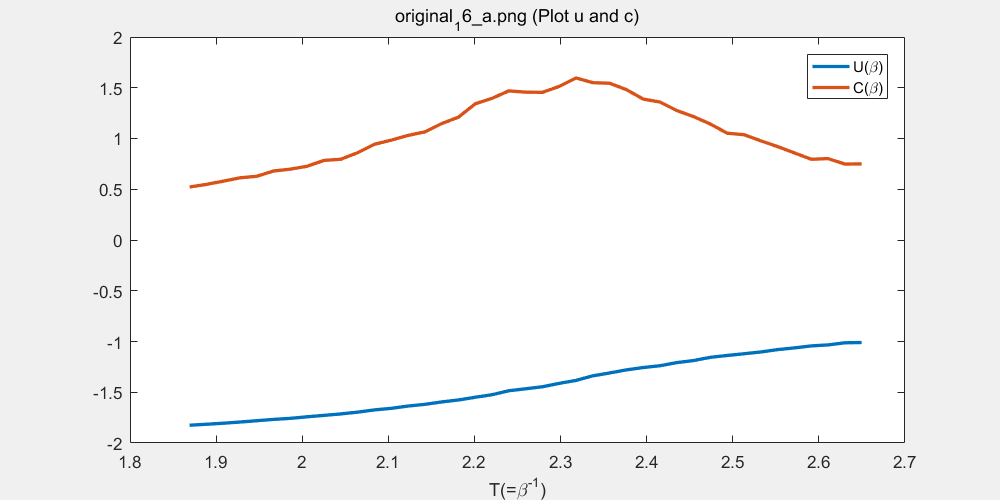
\includegraphics[width=0.45\paperwidth]{pics/original_16_a.png}
		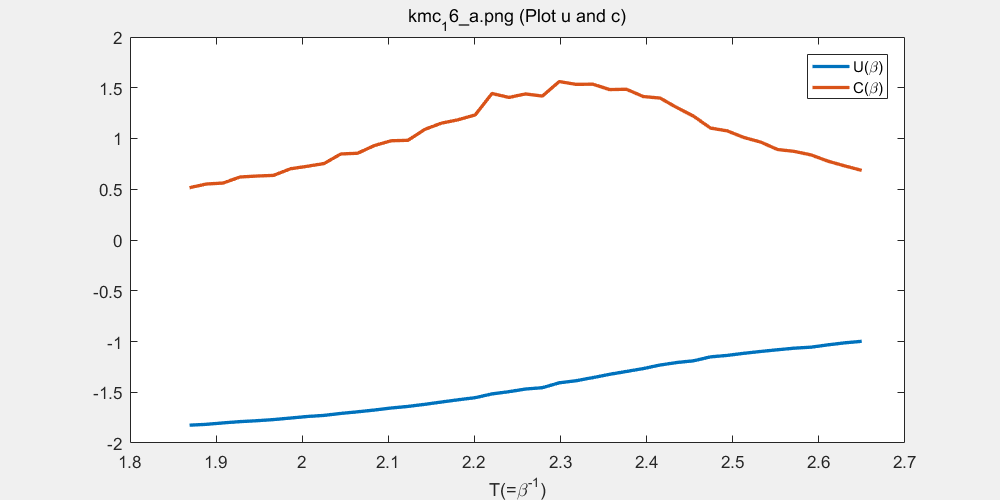
\includegraphics[width=0.45\paperwidth]{pics/kmc_16_a.png} }
	
	\noindent\makebox[\textwidth][c] {
		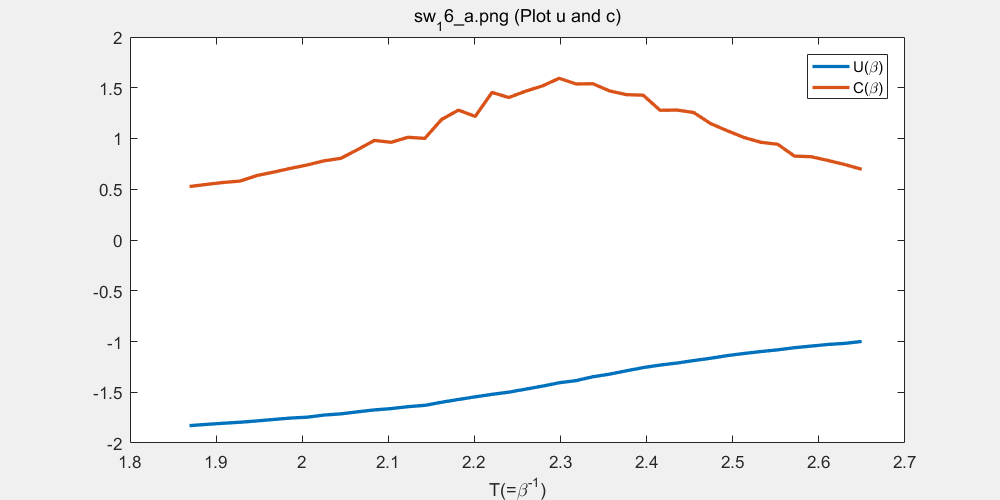
\includegraphics[width=0.45\paperwidth]{pics/sw_16_a.png}
		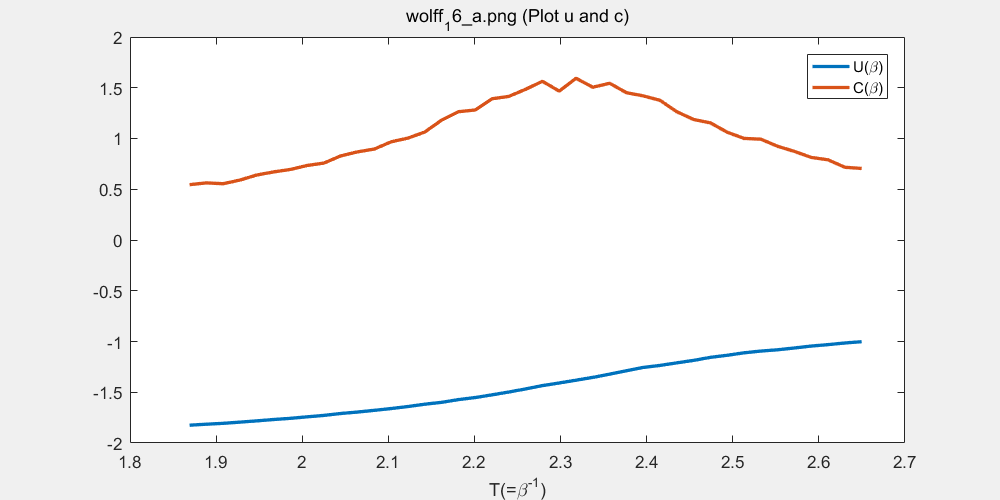
\includegraphics[width=0.45\paperwidth]{pics/wolff_16_a.png} }
\end{figure}

\begin{figure}[H]
	\centering
	\noindent\makebox[\textwidth][c] {
		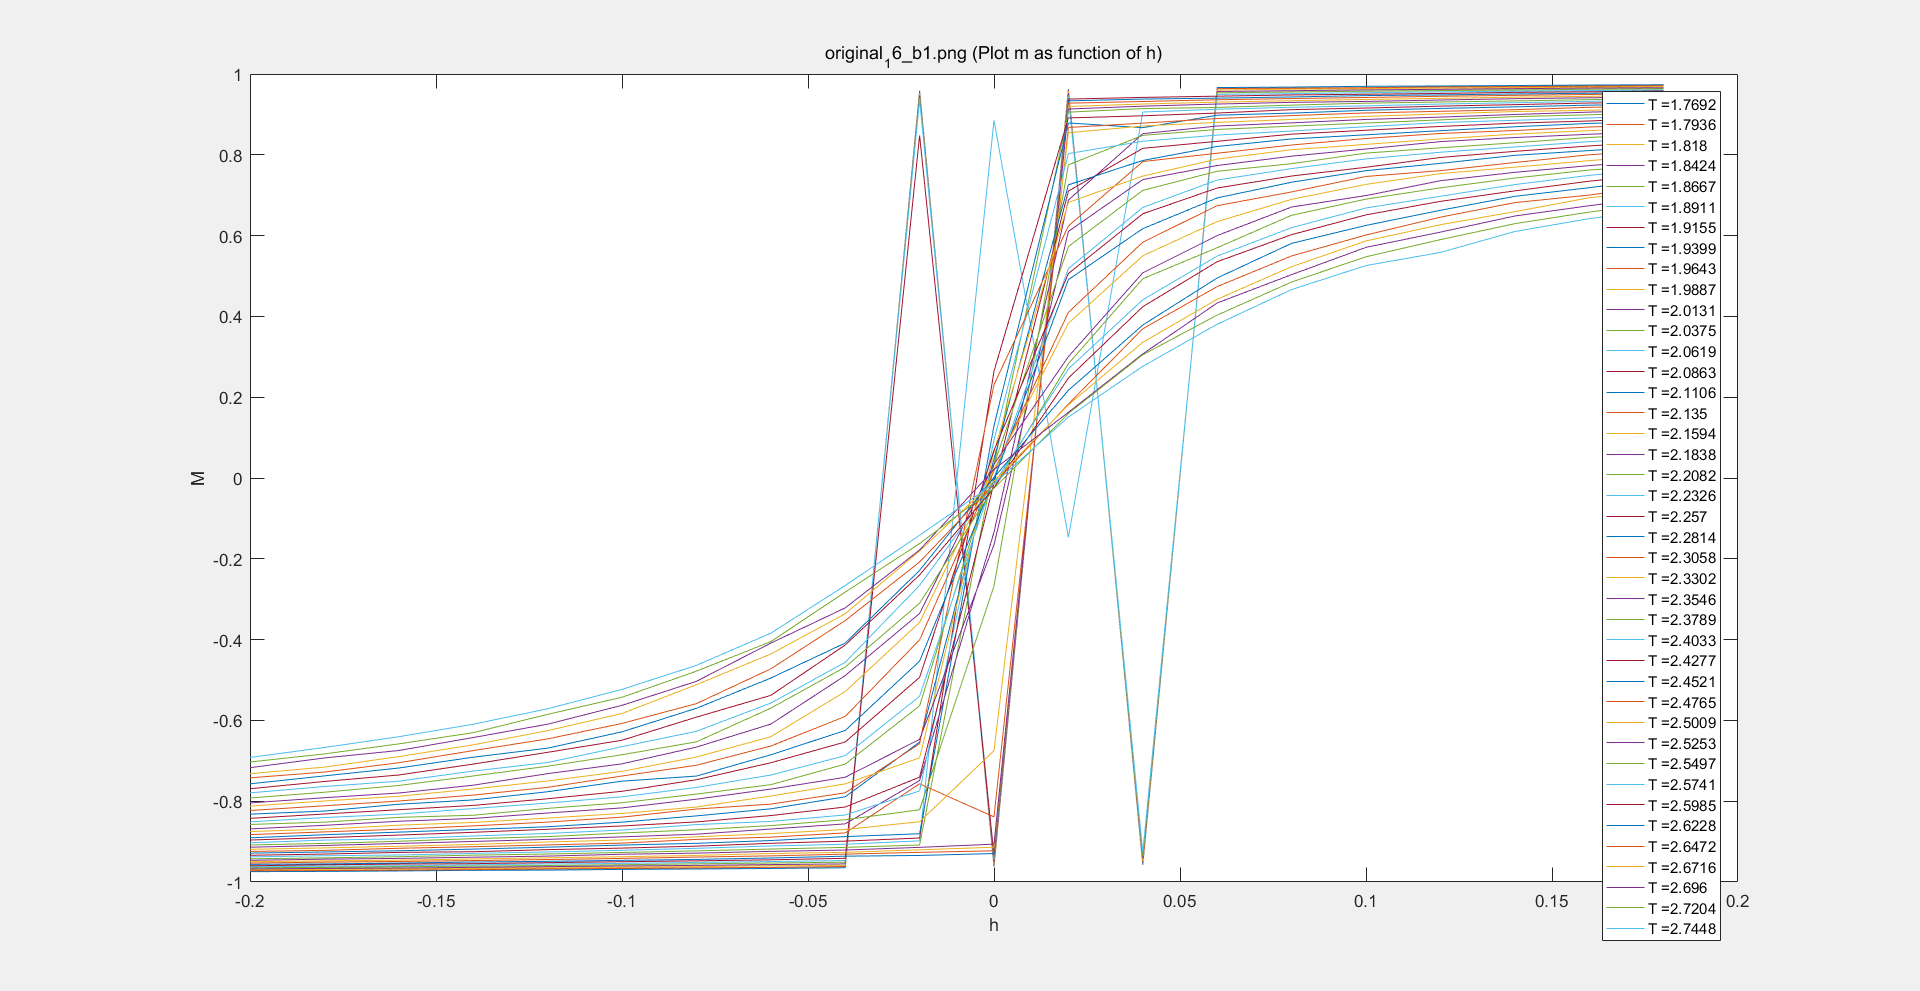
\includegraphics[width=0.45\paperwidth]{pics/original_16_b1.png}
		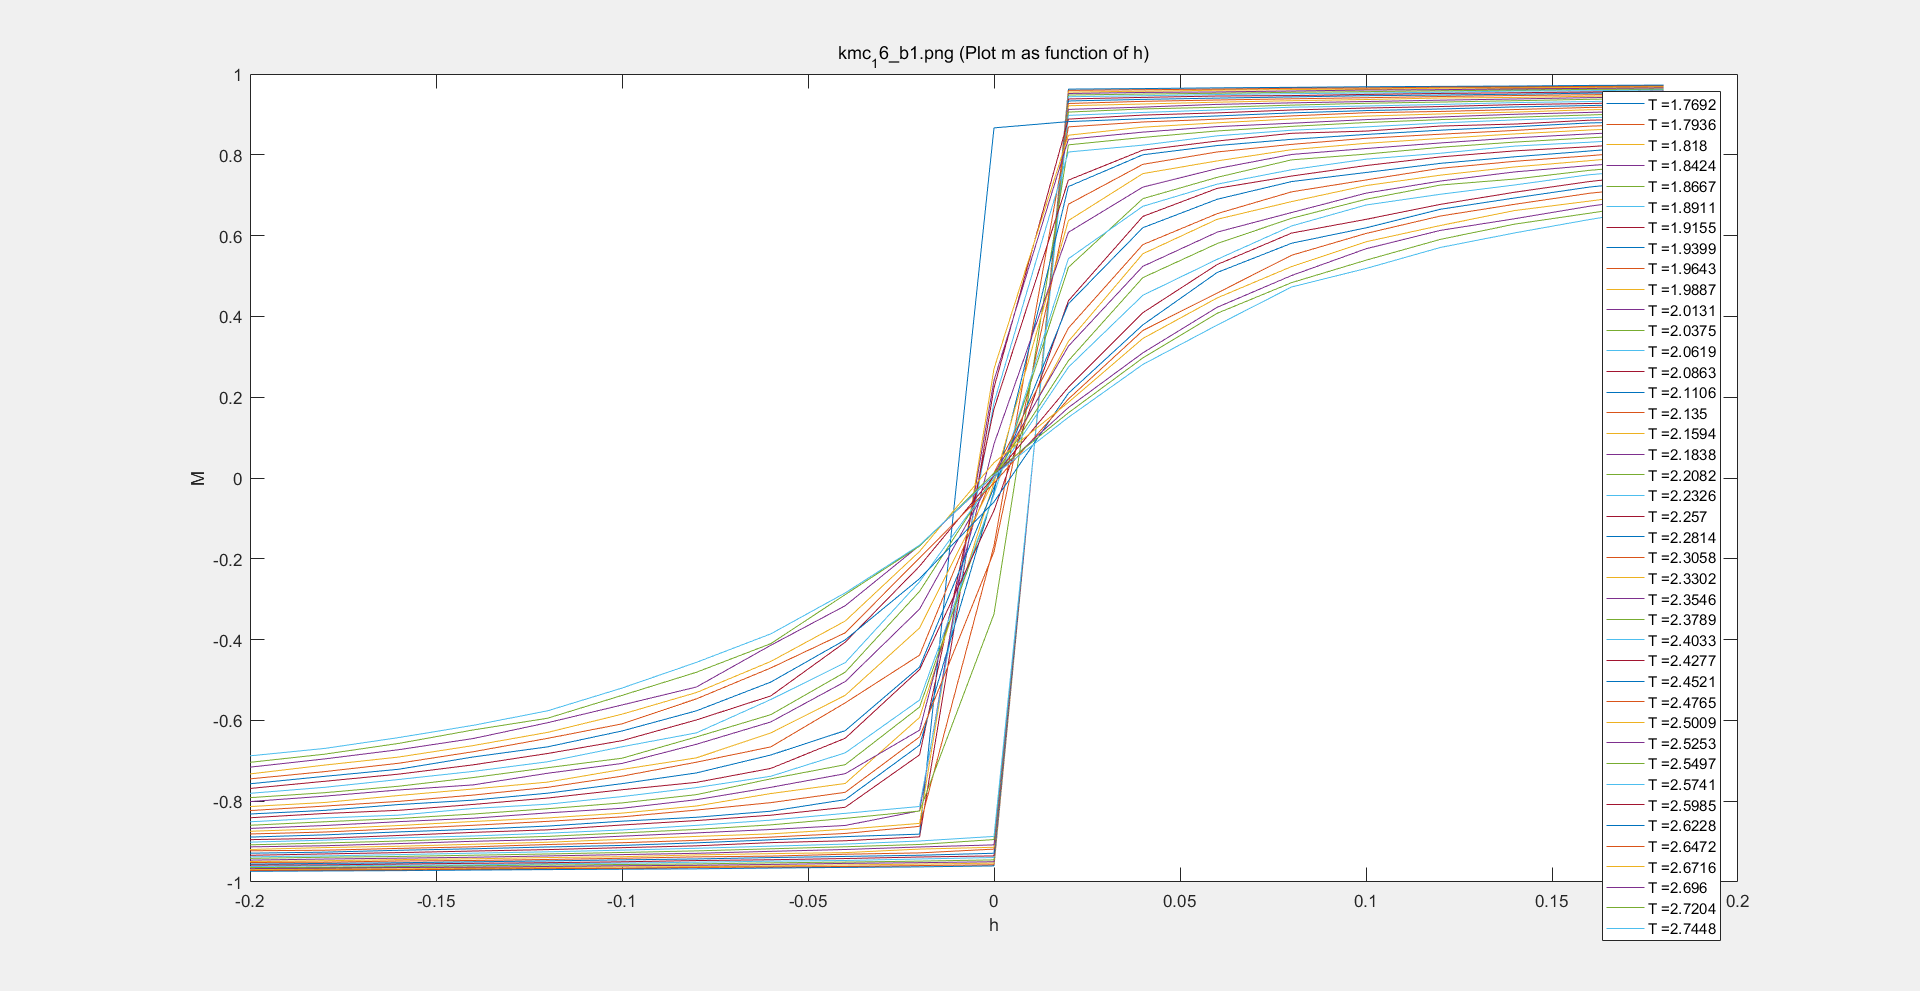
\includegraphics[width=0.45\paperwidth]{pics/kmc_16_b1.png} }
\end{figure}

\begin{figure}[H]
	\centering
	\noindent\makebox[\textwidth][c] {
		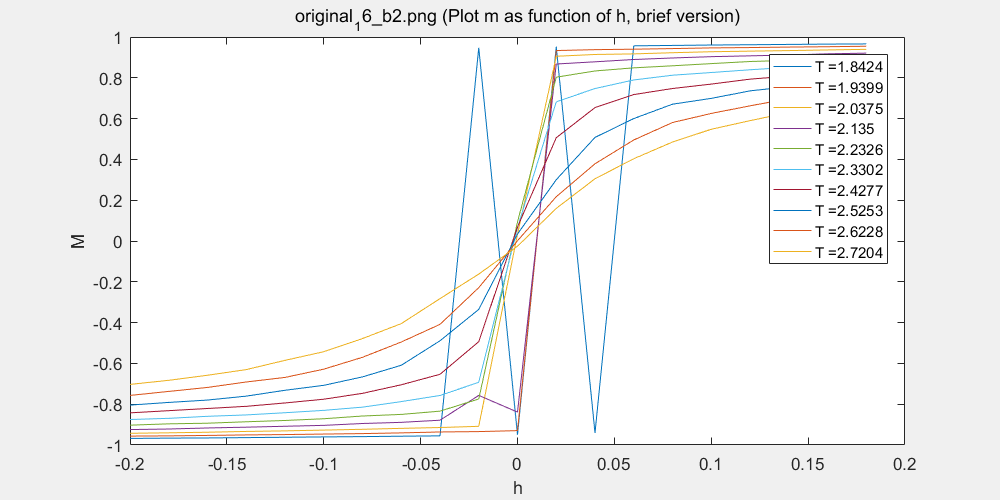
\includegraphics[width=0.45\paperwidth]{pics/original_16_b2.png}
		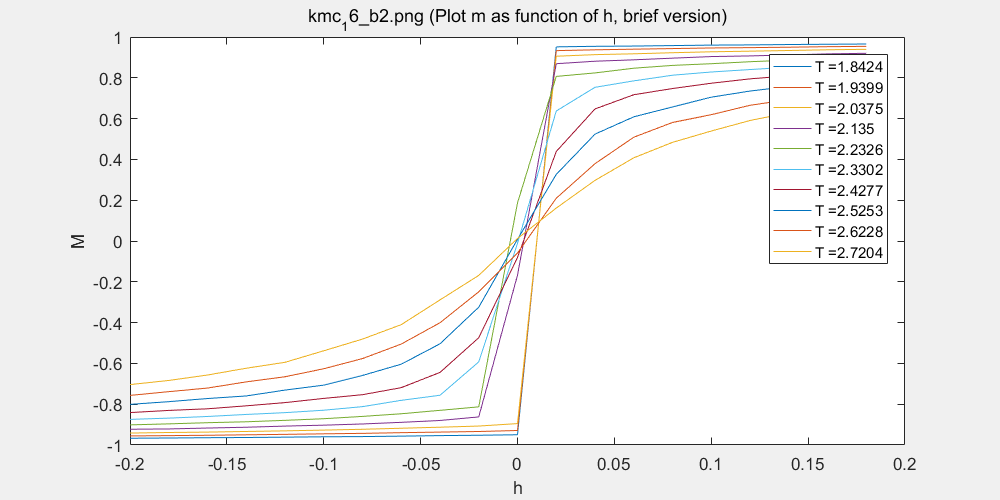
\includegraphics[width=0.45\paperwidth]{pics/kmc_16_b2.png} }
\end{figure}

\begin{figure}[H]
	\centering
	\noindent\makebox[\textwidth][c] {
		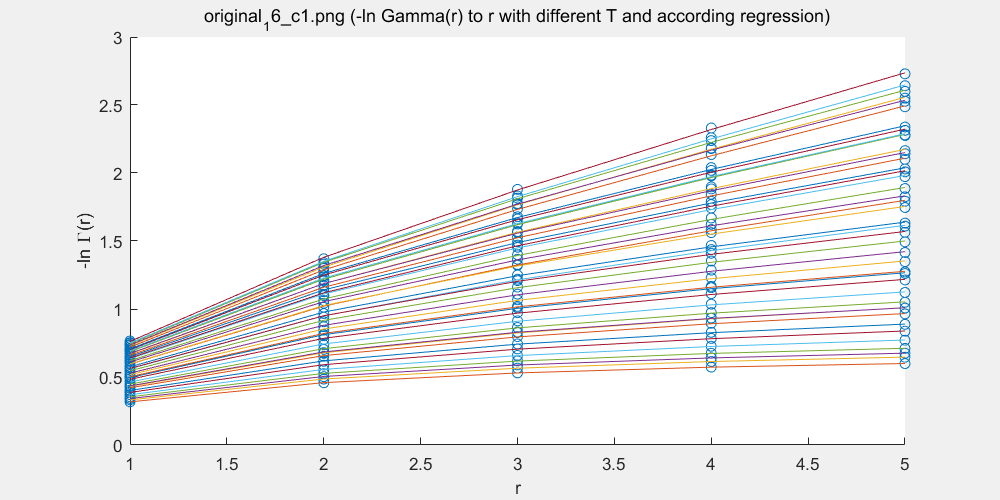
\includegraphics[width=0.45\paperwidth]{pics/original_16_c1.png}
		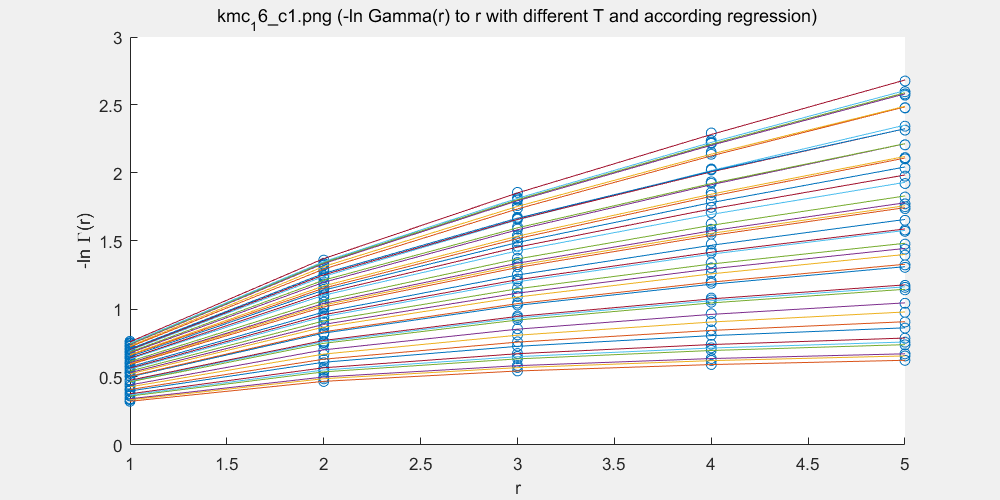
\includegraphics[width=0.45\paperwidth]{pics/kmc_16_c1.png} }
	
	\noindent\makebox[\textwidth][c] {
		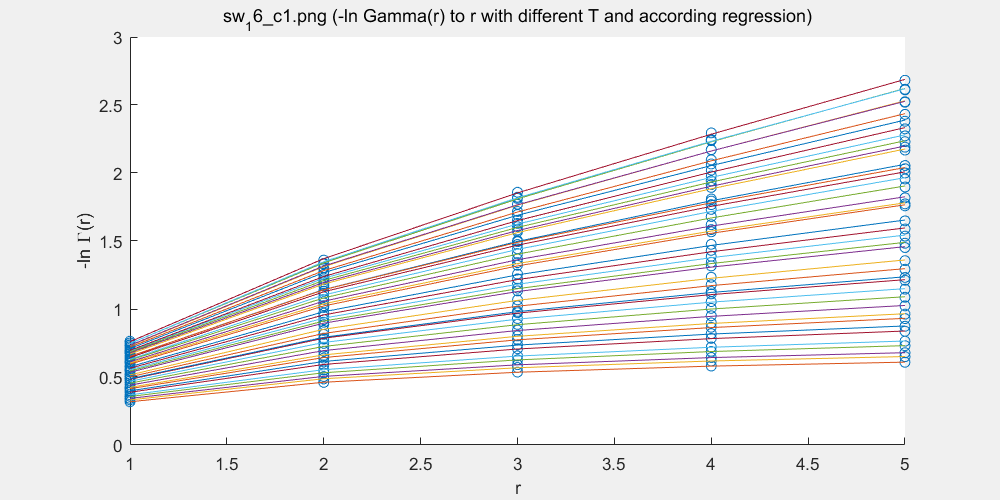
\includegraphics[width=0.45\paperwidth]{pics/sw_16_c1.png}
		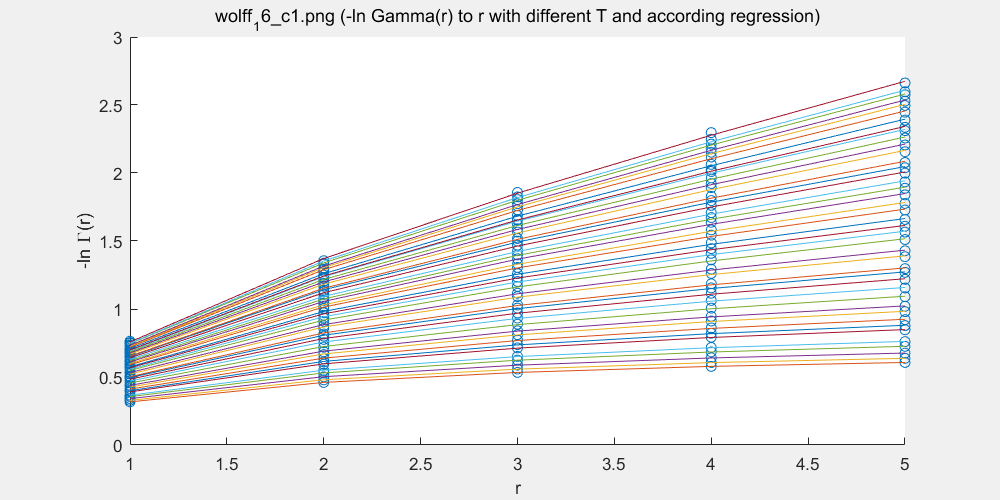
\includegraphics[width=0.45\paperwidth]{pics/wolff_16_c1.png} }
\end{figure}

\begin{figure}[H]
	\centering
	\noindent\makebox[\textwidth][c] {
		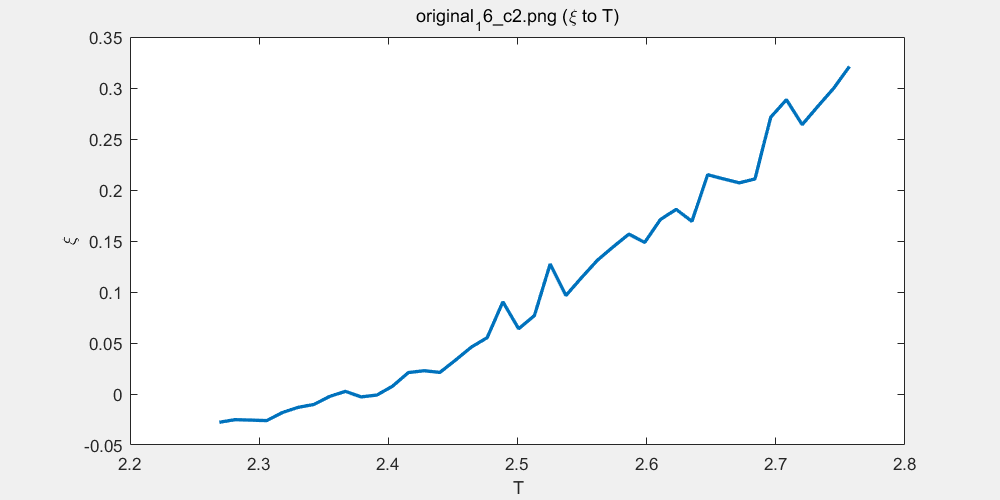
\includegraphics[width=0.45\paperwidth]{pics/original_16_c2.png}
		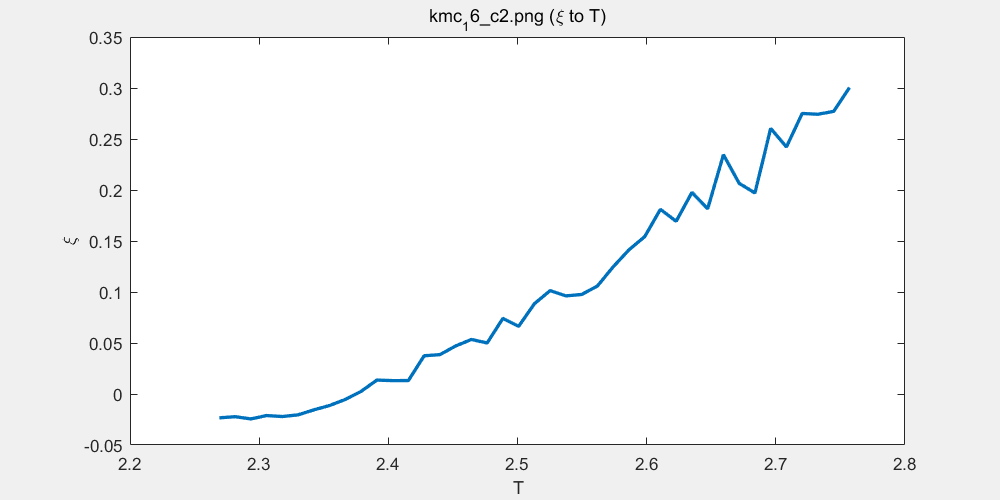
\includegraphics[width=0.45\paperwidth]{pics/kmc_16_c2.png} }
	
	\noindent\makebox[\textwidth][c] {
		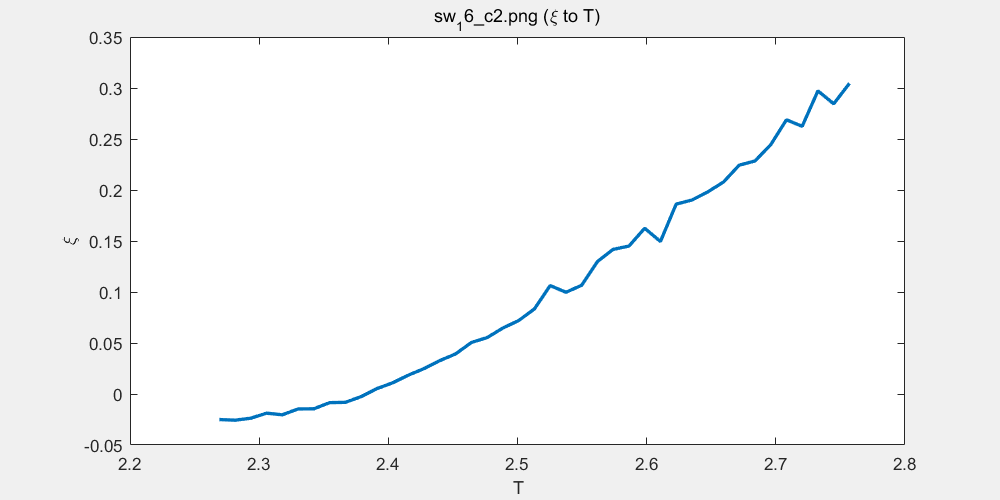
\includegraphics[width=0.45\paperwidth]{pics/sw_16_c2.png}
		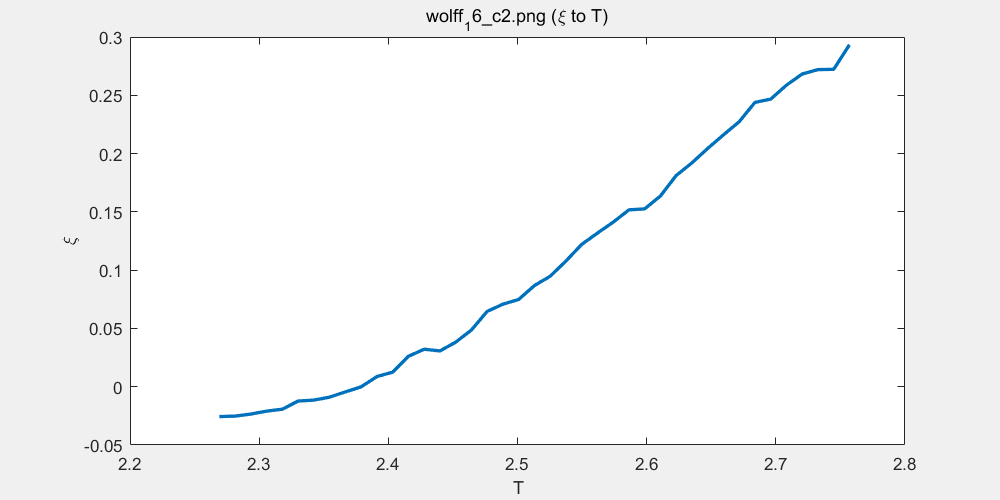
\includegraphics[width=0.45\paperwidth]{pics/wolff_16_c2.png} }
\end{figure}

\begin{figure}[H]
	\centering
	\noindent\makebox[\textwidth][c] {
		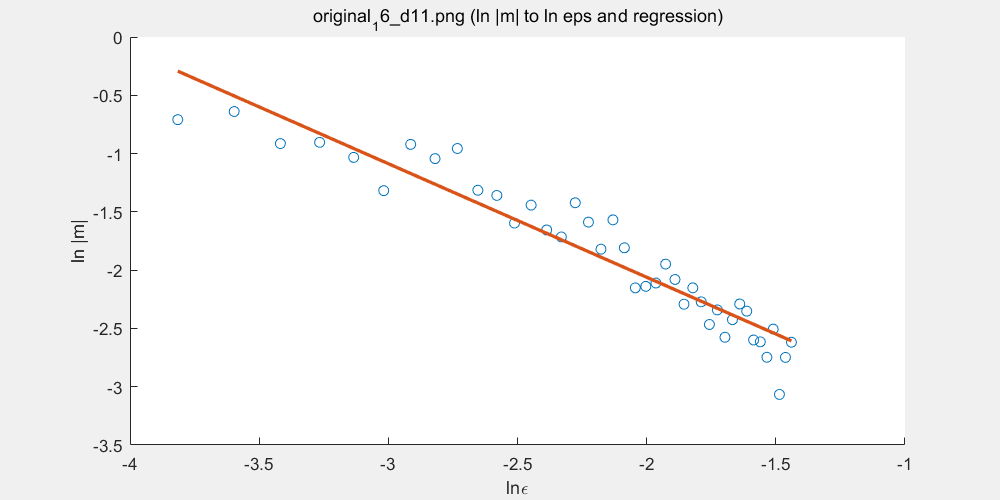
\includegraphics[width=0.45\paperwidth]{pics/original_16_d11.png}
		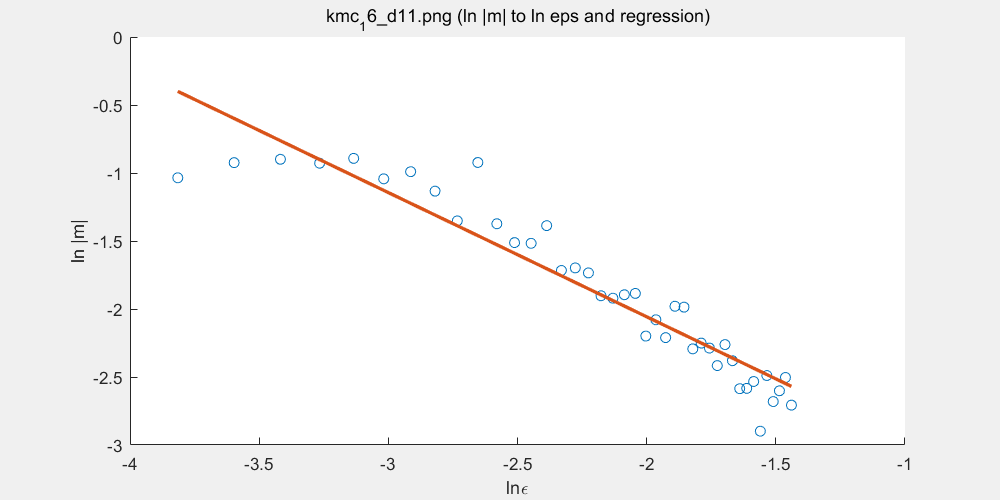
\includegraphics[width=0.45\paperwidth]{pics/kmc_16_d11.png} }
\end{figure}

\begin{figure}[H]
	\centering
	\noindent\makebox[\textwidth][c] {
		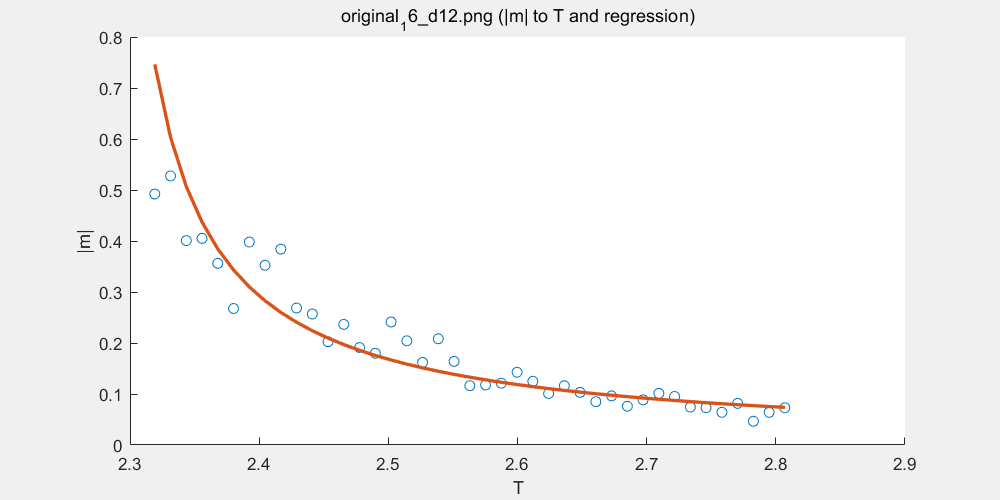
\includegraphics[width=0.45\paperwidth]{pics/original_16_d12.png}
		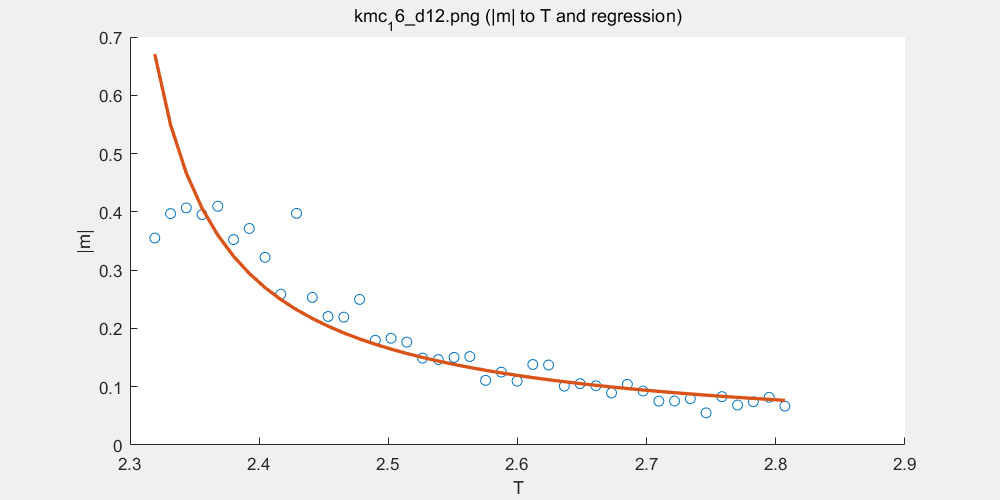
\includegraphics[width=0.45\paperwidth]{pics/kmc_16_d12.png} }
\end{figure}

\begin{figure}[H]
	\centering
	\noindent\makebox[\textwidth][c] {
		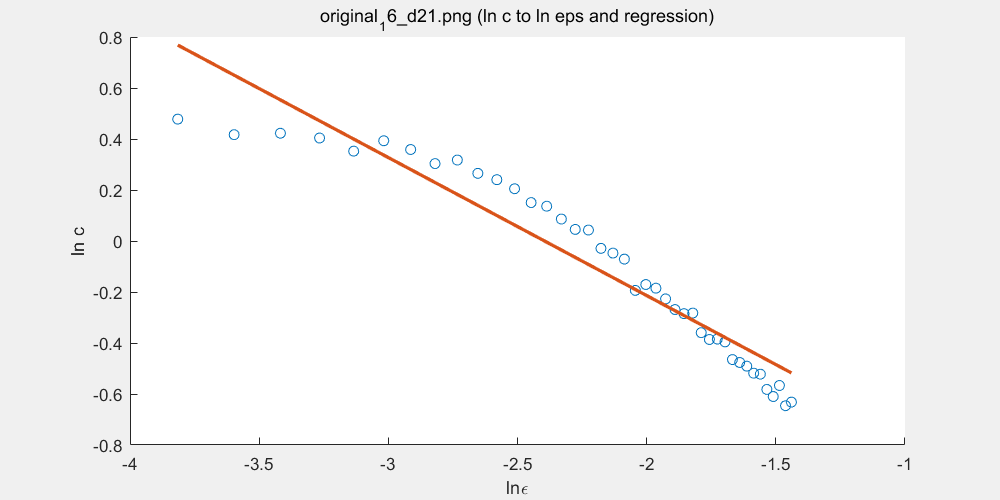
\includegraphics[width=0.45\paperwidth]{pics/original_16_d21.png}
		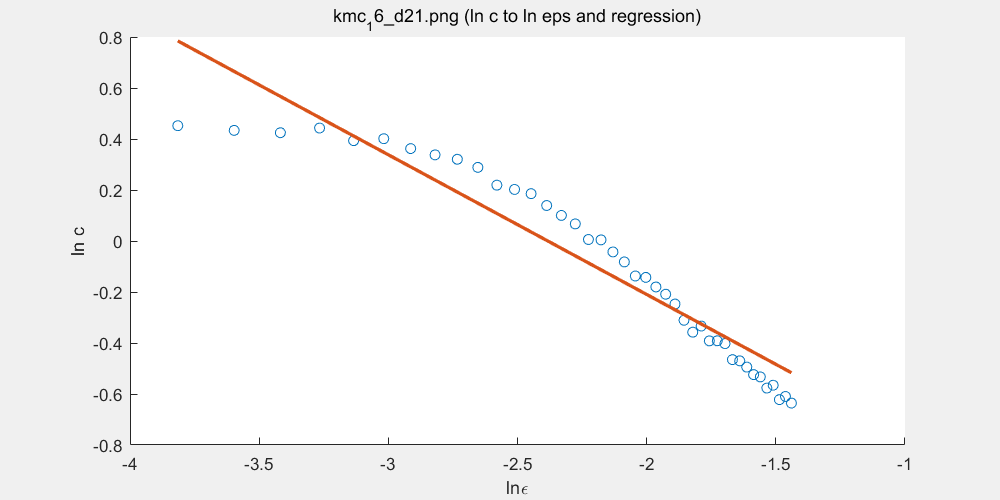
\includegraphics[width=0.45\paperwidth]{pics/kmc_16_d21.png} }
	
	\noindent\makebox[\textwidth][c] {
		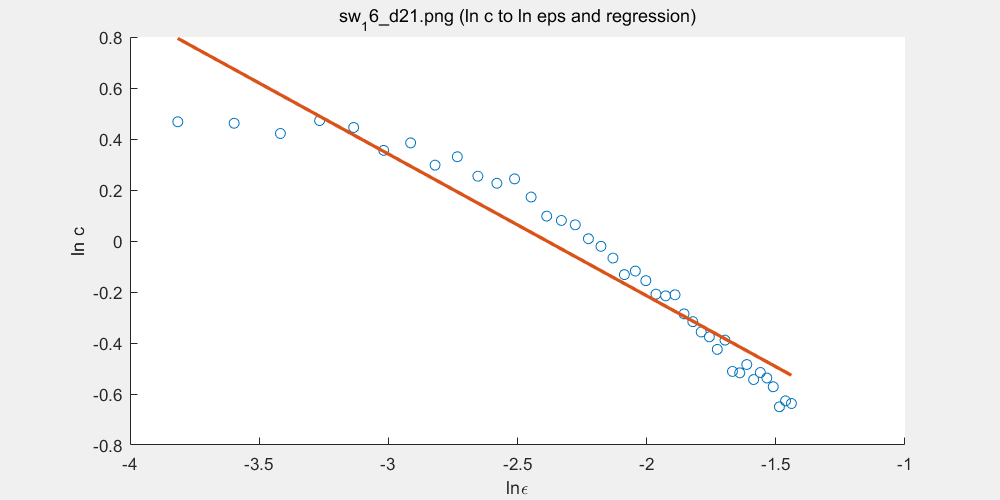
\includegraphics[width=0.45\paperwidth]{pics/sw_16_d21.png}
		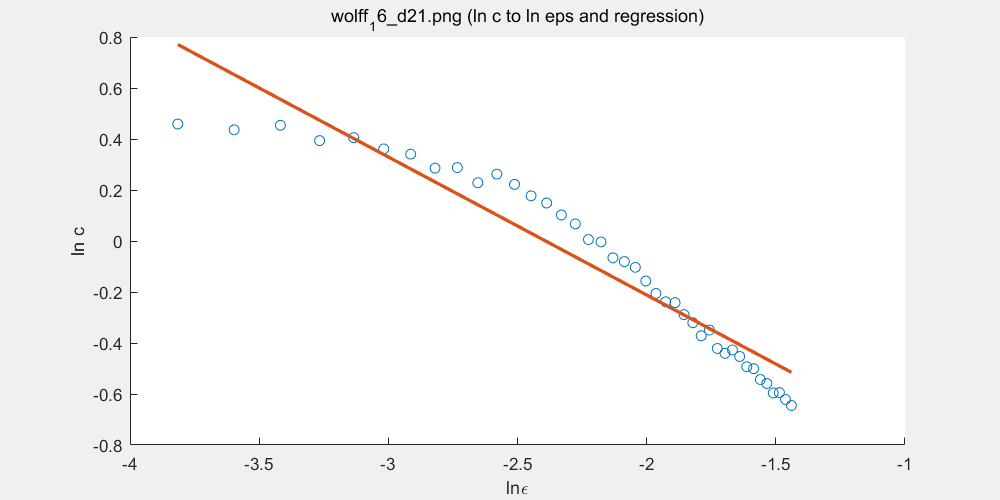
\includegraphics[width=0.45\paperwidth]{pics/wolff_16_d21.png} }
\end{figure}

\begin{figure}[H]
	\centering
	\noindent\makebox[\textwidth][c] {
		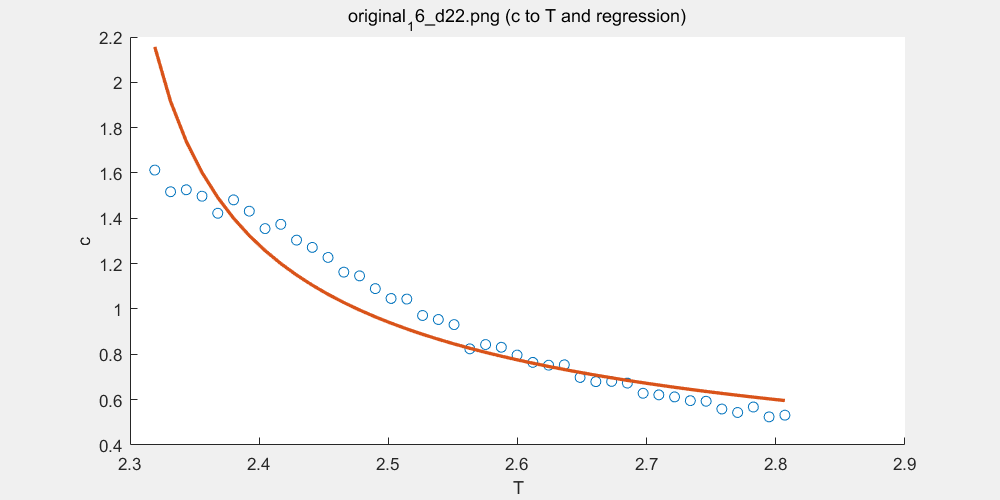
\includegraphics[width=0.45\paperwidth]{pics/original_16_d22.png}
		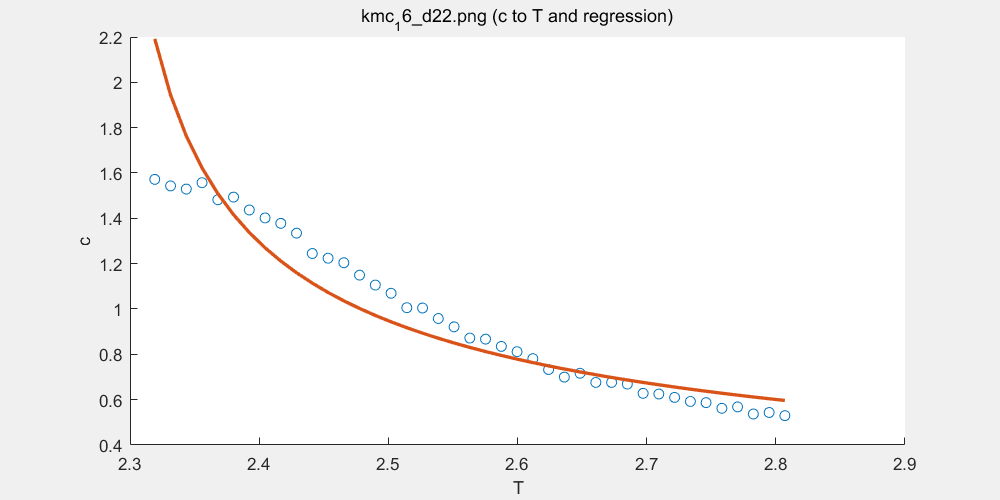
\includegraphics[width=0.45\paperwidth]{pics/kmc_16_d22.png} }
	
	\noindent\makebox[\textwidth][c] {
		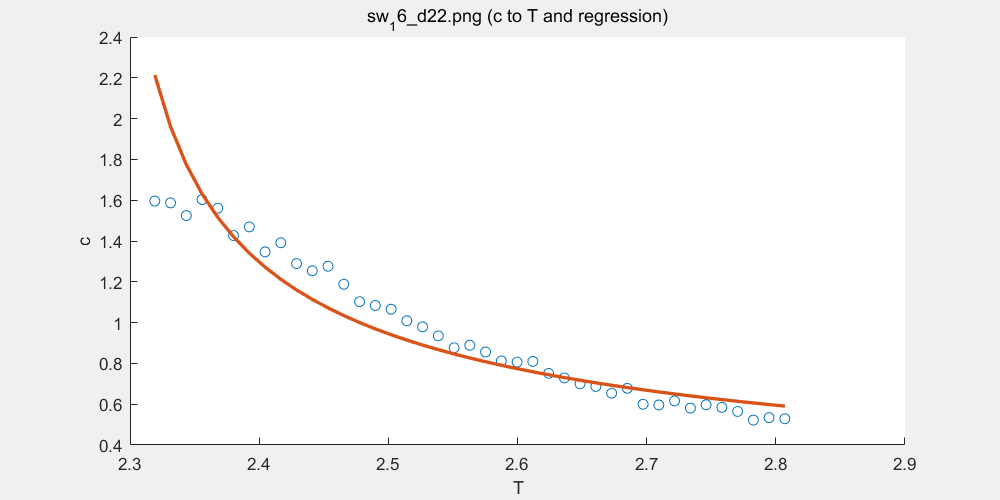
\includegraphics[width=0.45\paperwidth]{pics/sw_16_d22.png}
		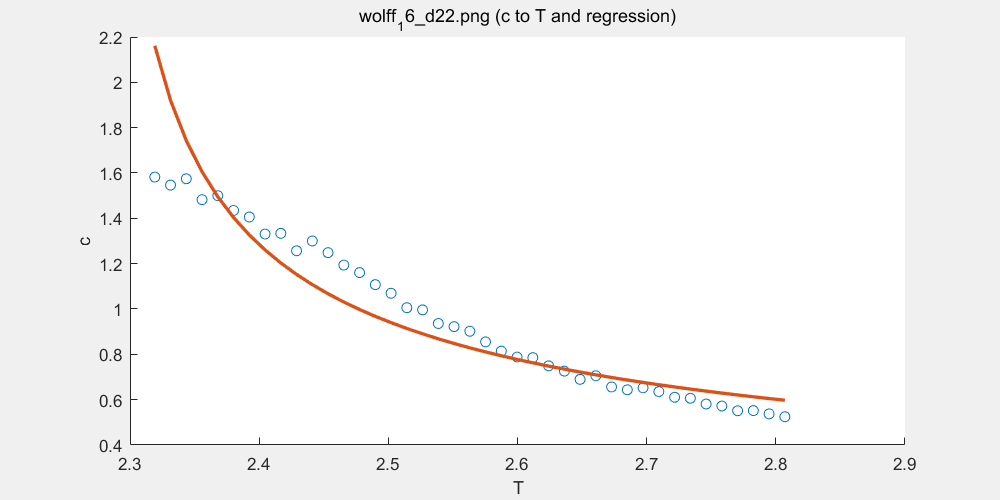
\includegraphics[width=0.45\paperwidth]{pics/wolff_16_d22.png} }
\end{figure}

\begin{figure}[H]
	\centering
	\noindent\makebox[\textwidth][c] {
		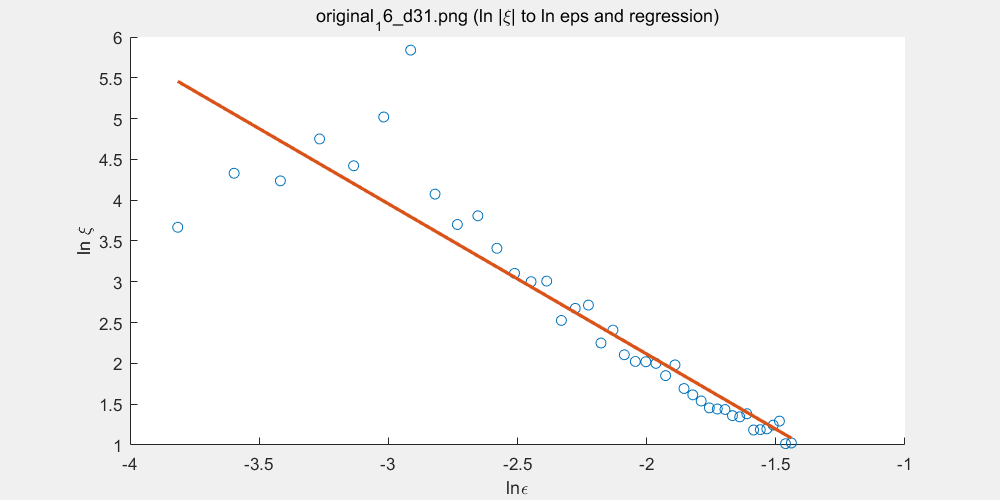
\includegraphics[width=0.45\paperwidth]{pics/original_16_d31.png}
		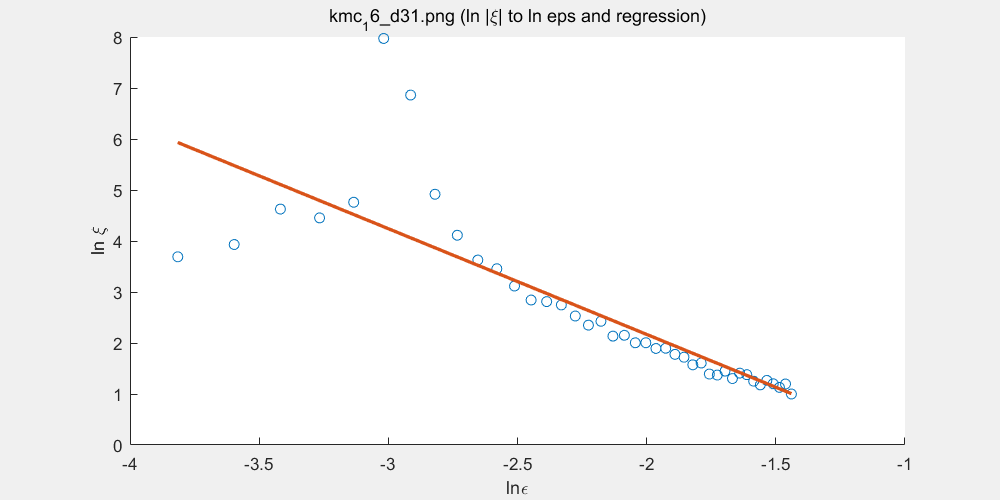
\includegraphics[width=0.45\paperwidth]{pics/kmc_16_d31.png} }
	
	\noindent\makebox[\textwidth][c] {
		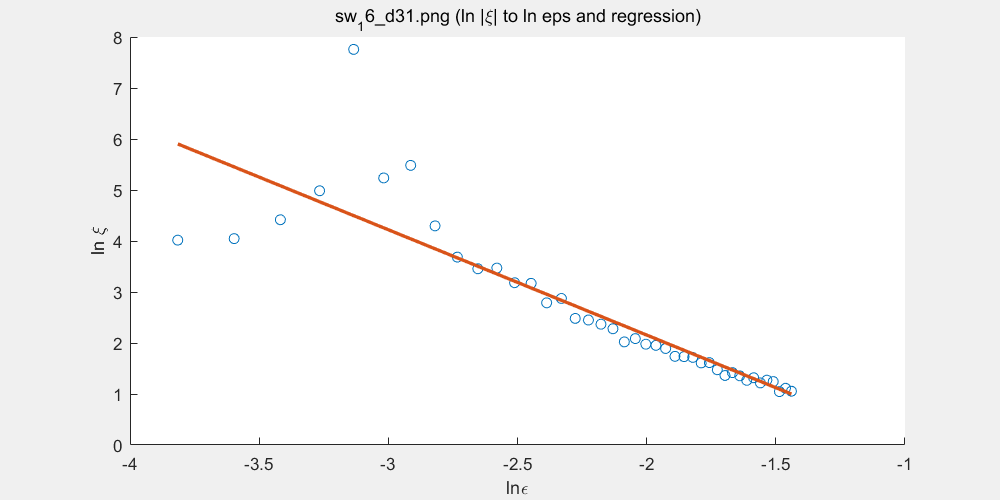
\includegraphics[width=0.45\paperwidth]{pics/sw_16_d31.png}
		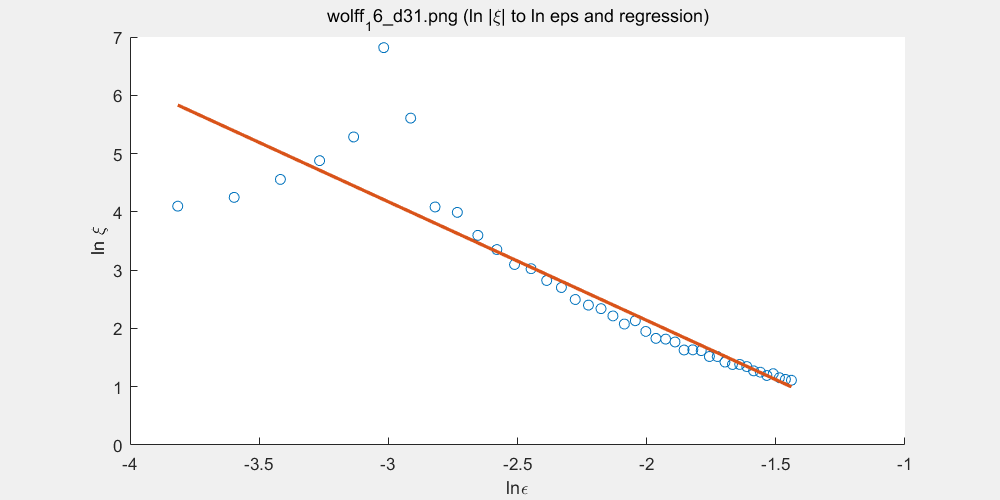
\includegraphics[width=0.45\paperwidth]{pics/wolff_16_d31.png} }
\end{figure}

\begin{figure}[H]
	\centering
	\noindent\makebox[\textwidth][c] {
		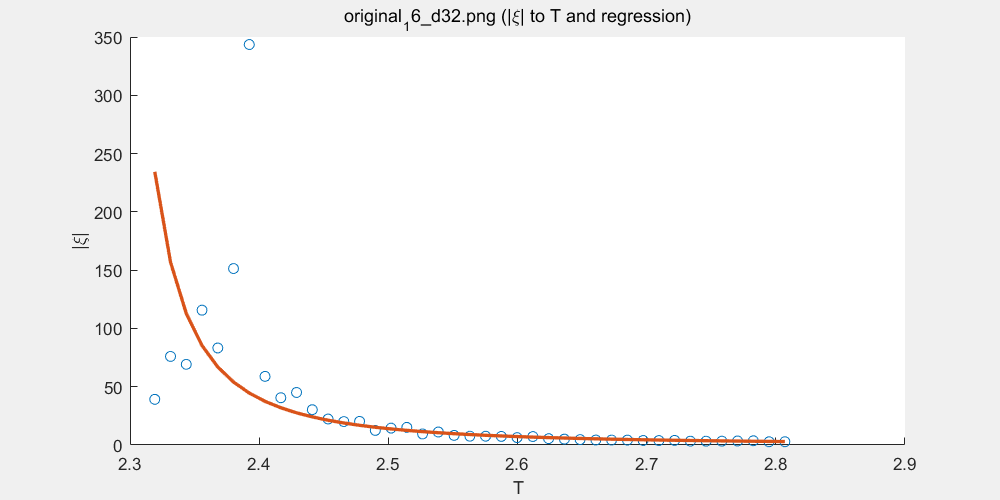
\includegraphics[width=0.45\paperwidth]{pics/original_16_d32.png}
		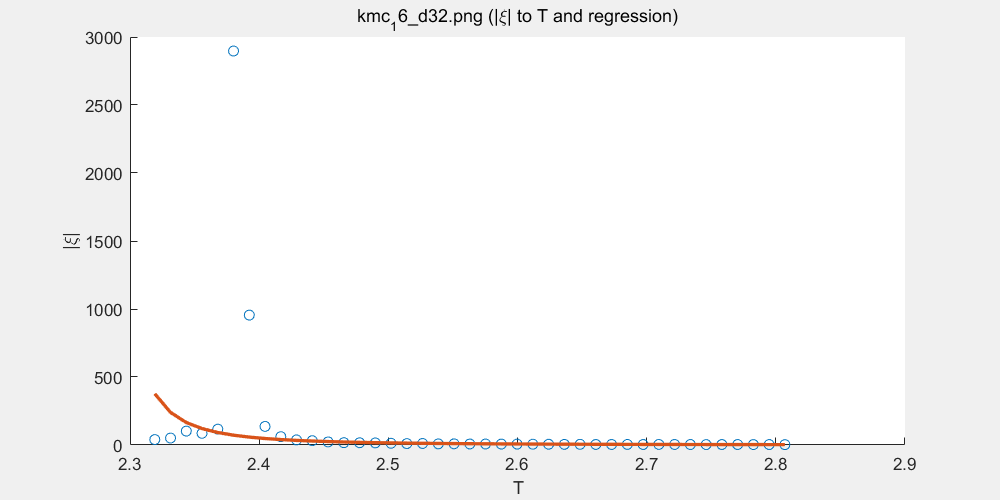
\includegraphics[width=0.45\paperwidth]{pics/kmc_16_d32.png} }
	
	\noindent\makebox[\textwidth][c] {
		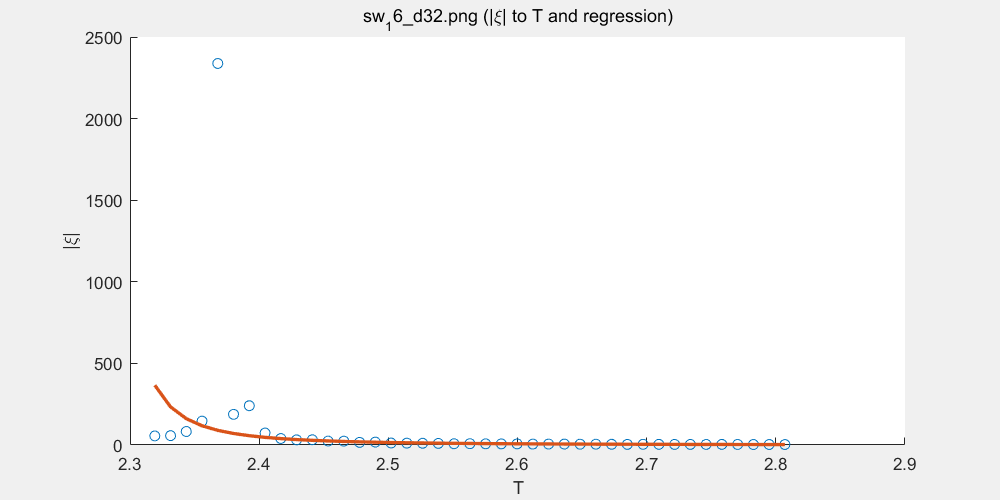
\includegraphics[width=0.45\paperwidth]{pics/sw_16_d32.png}
		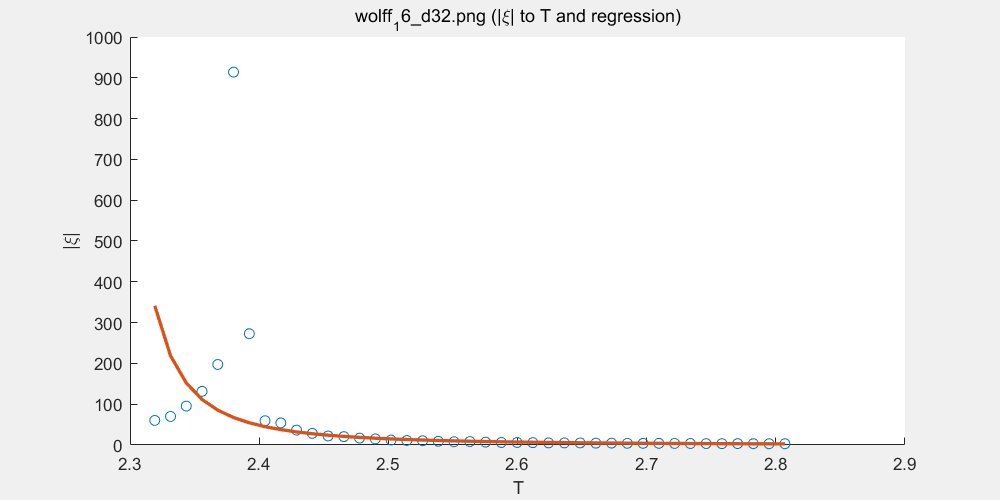
\includegraphics[width=0.45\paperwidth]{pics/wolff_16_d32.png} }
\end{figure}

\subsection{$N=32$}
\begin{figure}[H]
	\centering
	\noindent\makebox[\textwidth][c] {
		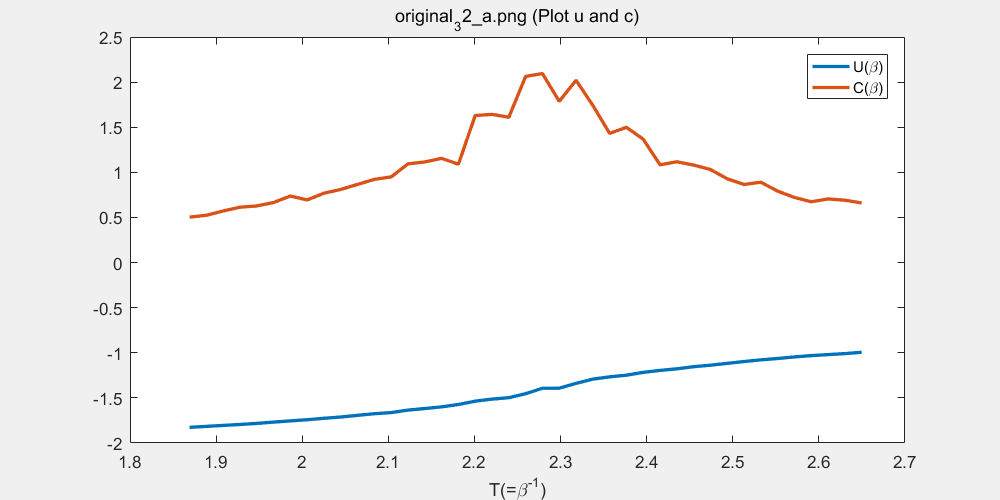
\includegraphics[width=0.45\paperwidth]{pics/original_32_a.png}
		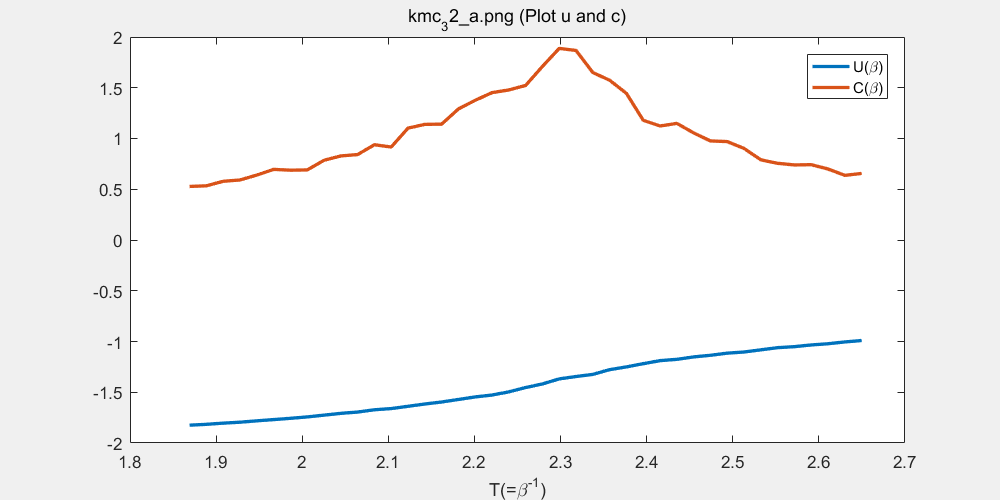
\includegraphics[width=0.45\paperwidth]{pics/kmc_32_a.png} }
	
	\noindent\makebox[\textwidth][c] {
		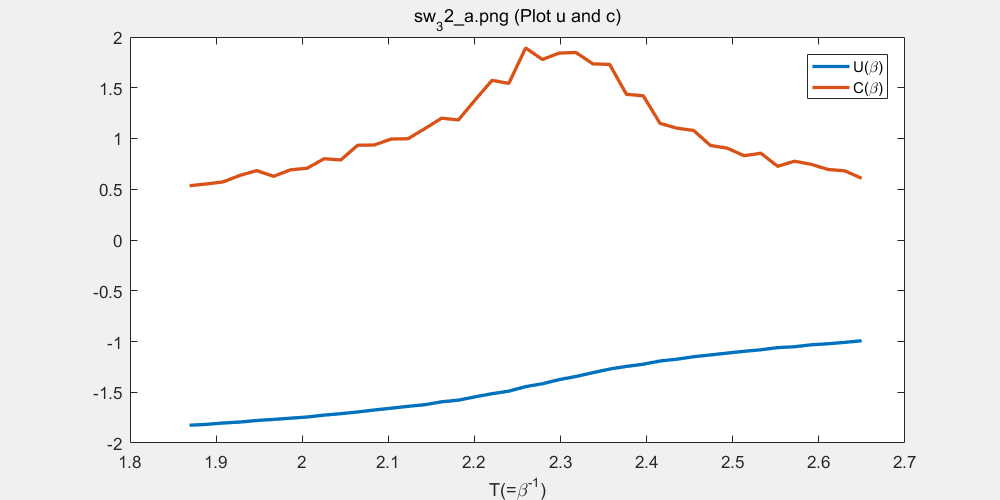
\includegraphics[width=0.45\paperwidth]{pics/sw_32_a.png}
		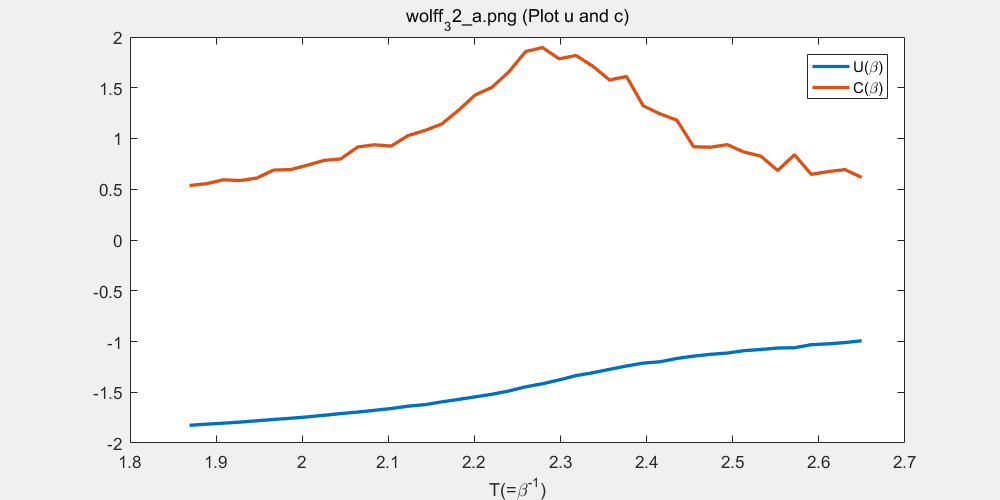
\includegraphics[width=0.45\paperwidth]{pics/wolff_32_a.png} }
\end{figure}

\begin{figure}[H]
	\centering
	\noindent\makebox[\textwidth][c] {
		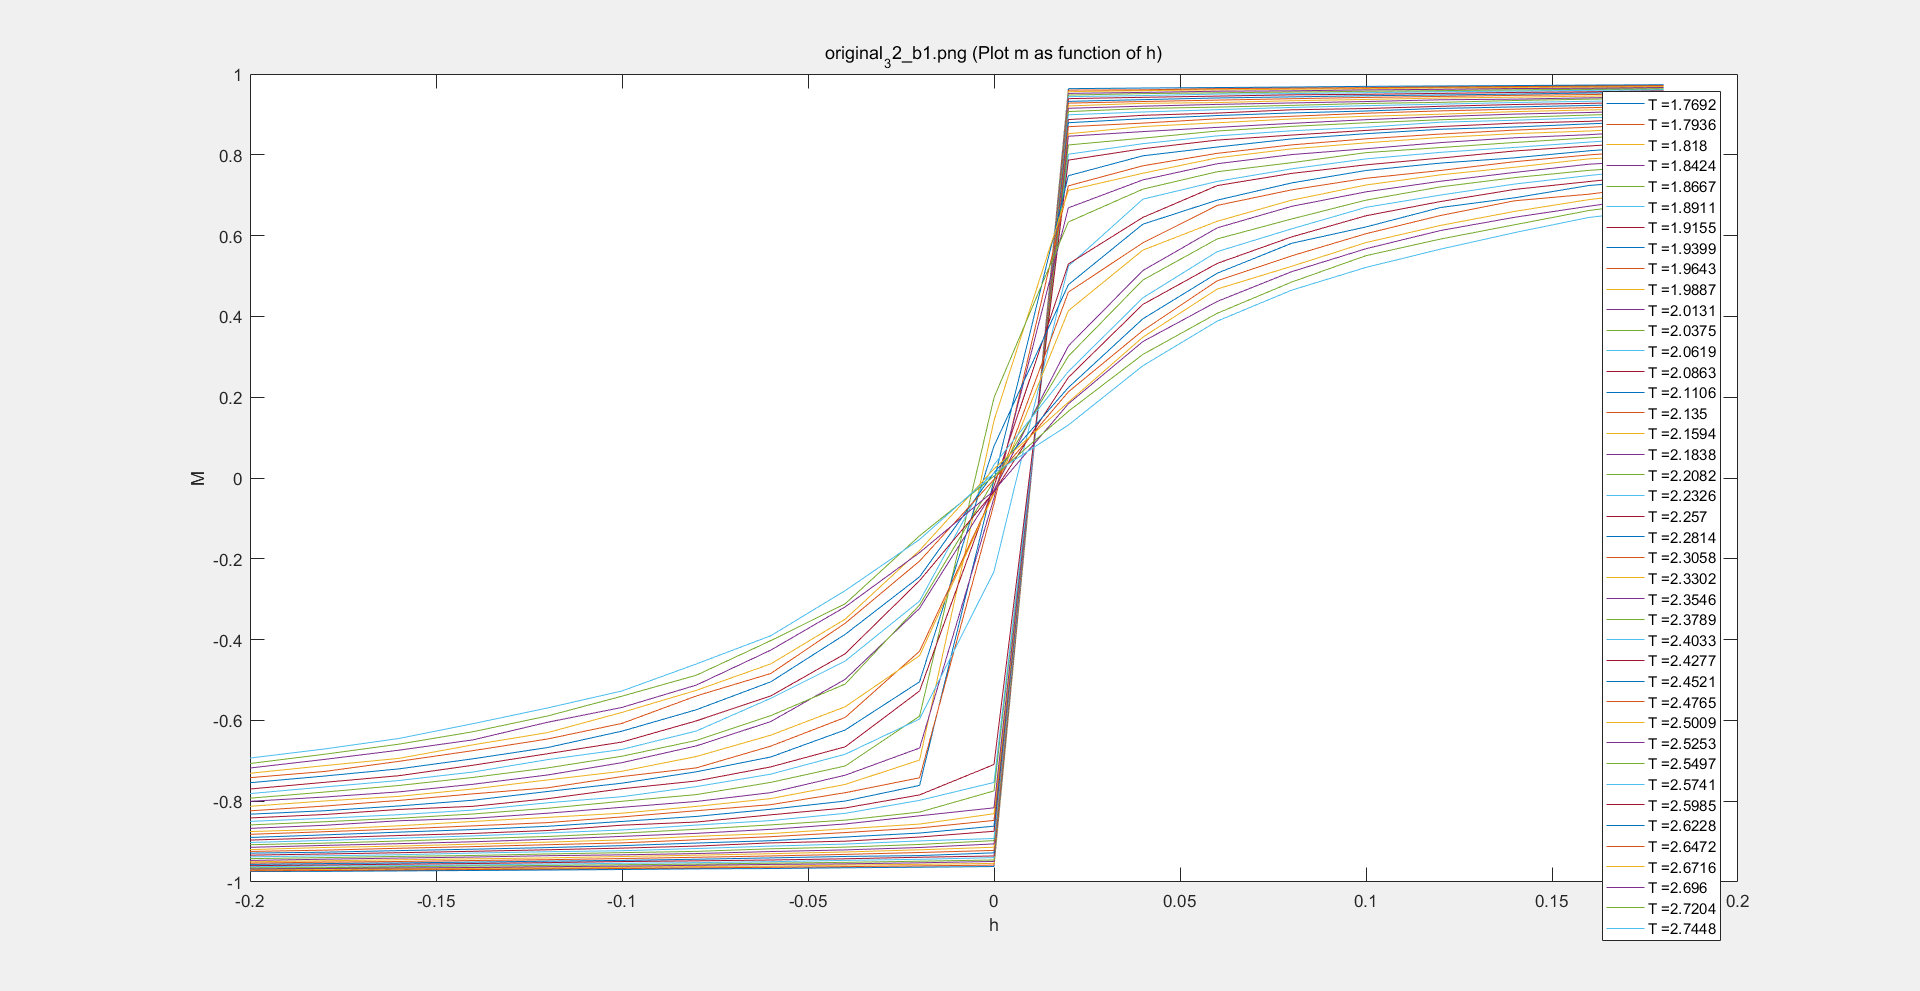
\includegraphics[width=0.45\paperwidth]{pics/original_32_b1.png}
		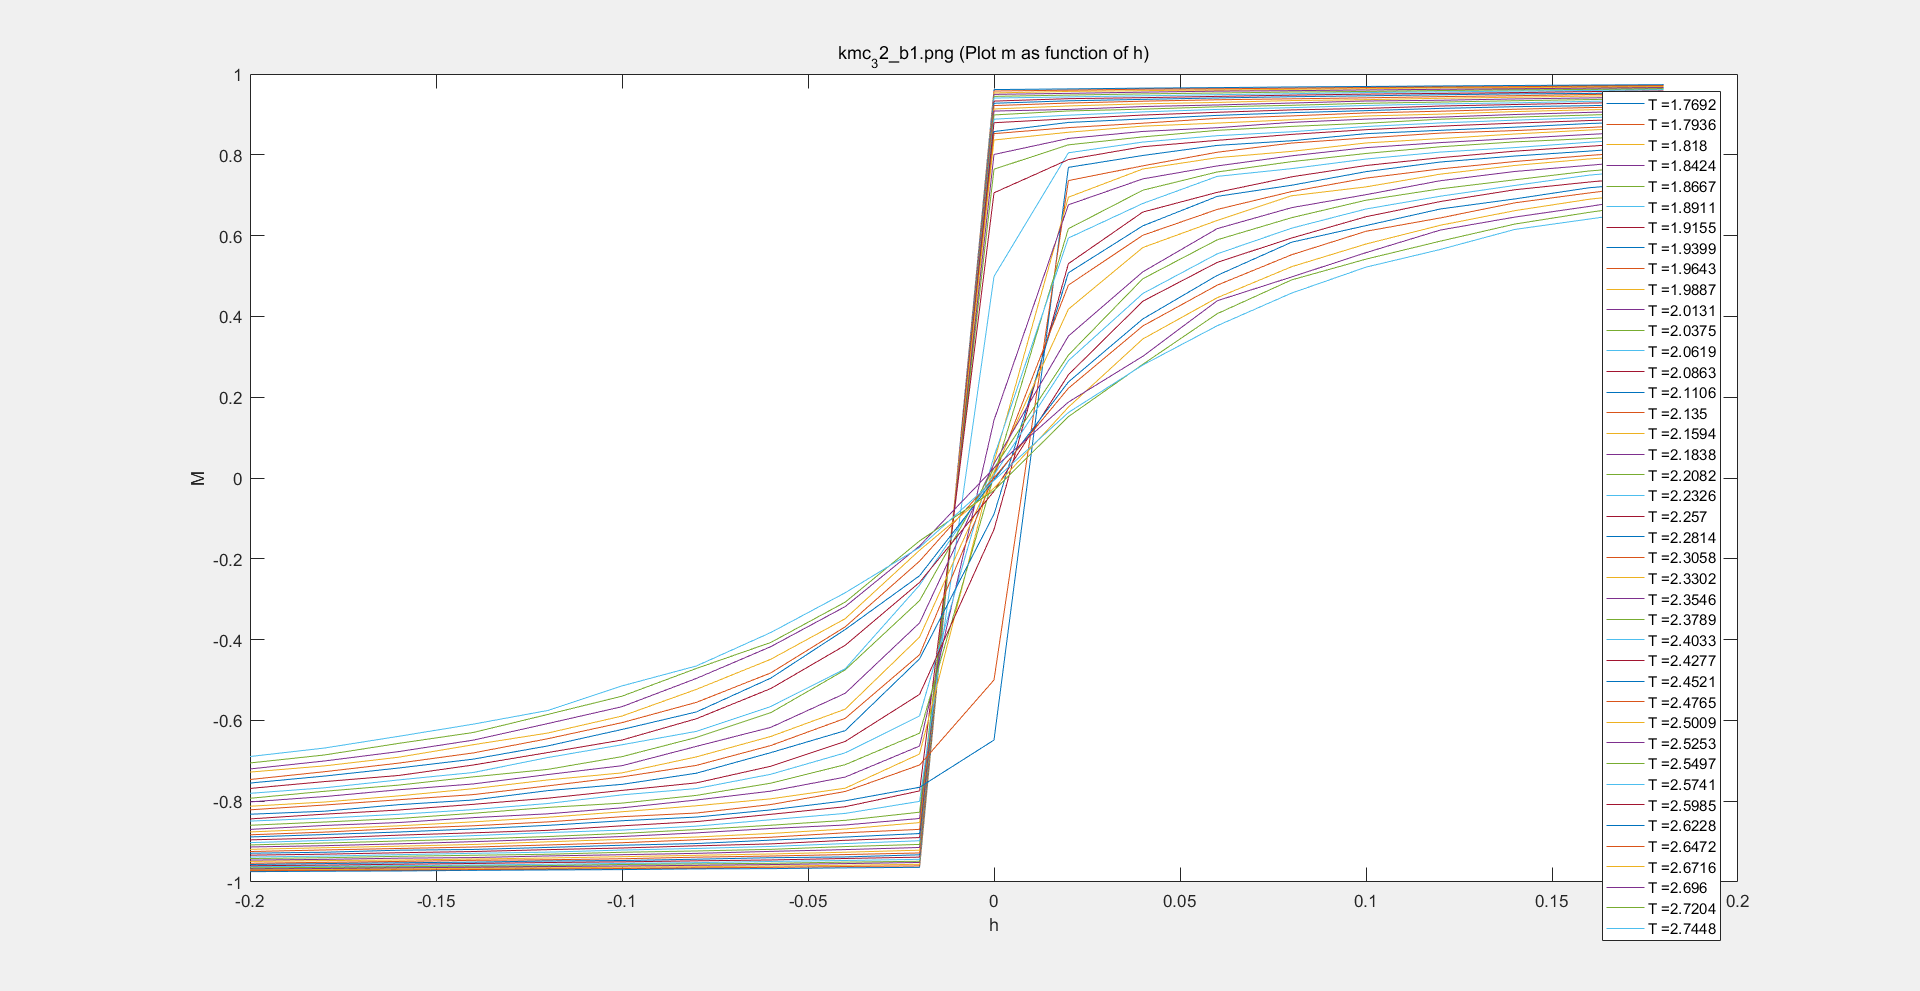
\includegraphics[width=0.45\paperwidth]{pics/kmc_32_b1.png} }
\end{figure}

\begin{figure}[H]
	\centering
	\noindent\makebox[\textwidth][c] {
		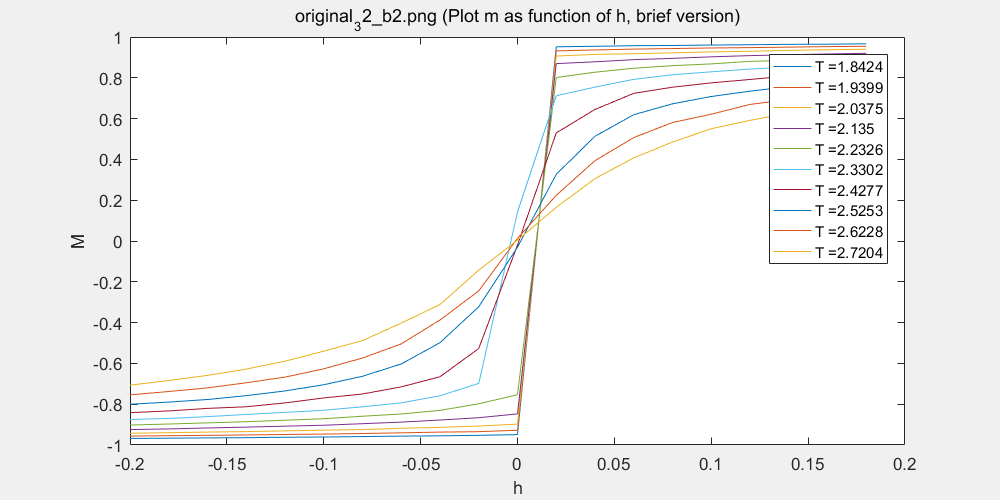
\includegraphics[width=0.45\paperwidth]{pics/original_32_b2.png}
		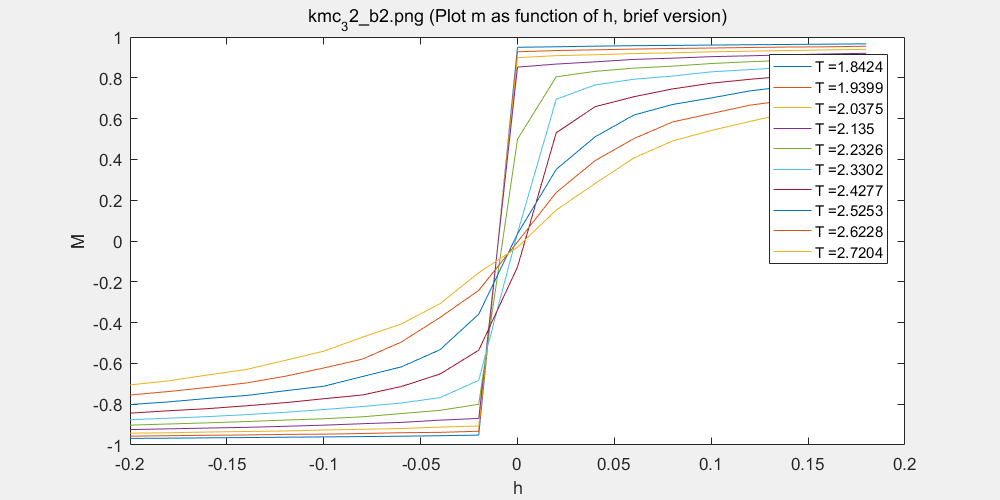
\includegraphics[width=0.45\paperwidth]{pics/kmc_32_b2.png} }
\end{figure}

\begin{figure}[H]
	\centering
	\noindent\makebox[\textwidth][c] {
		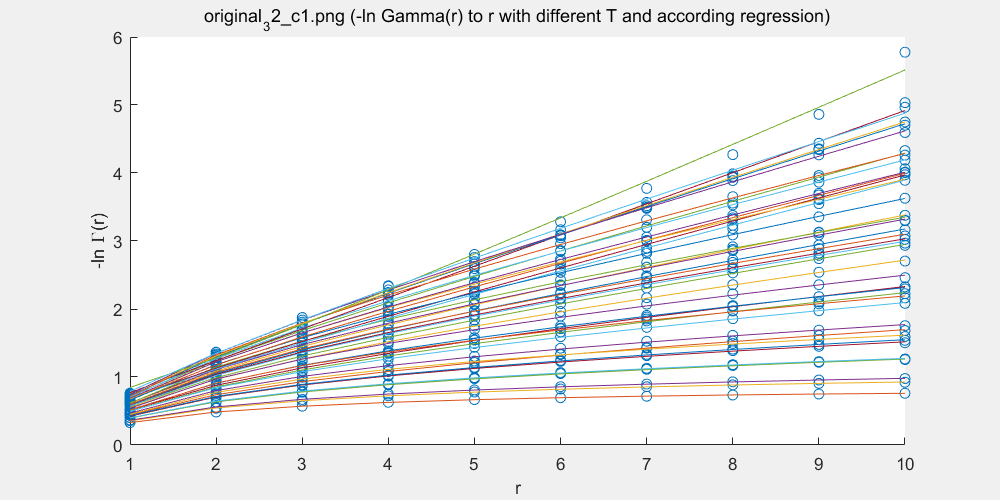
\includegraphics[width=0.45\paperwidth]{pics/original_32_c1.png}
		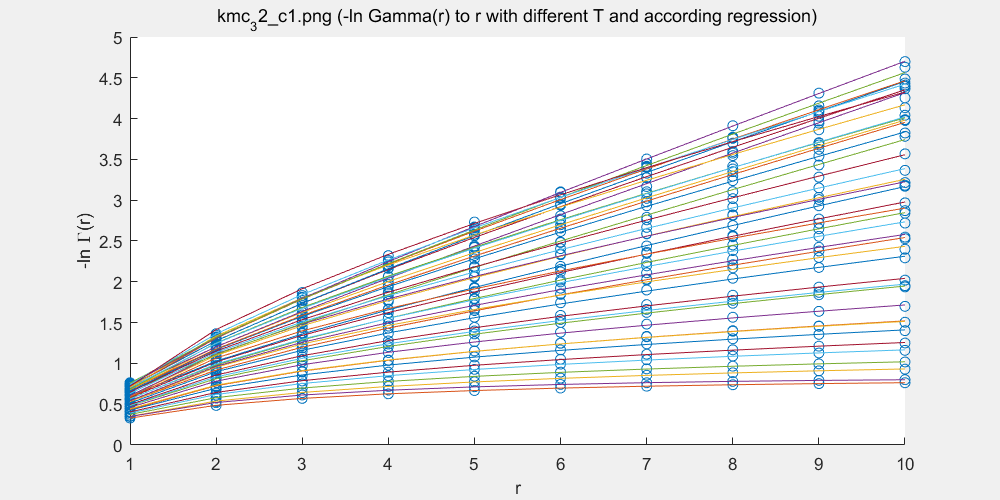
\includegraphics[width=0.45\paperwidth]{pics/kmc_32_c1.png} }
	
	\noindent\makebox[\textwidth][c] {
		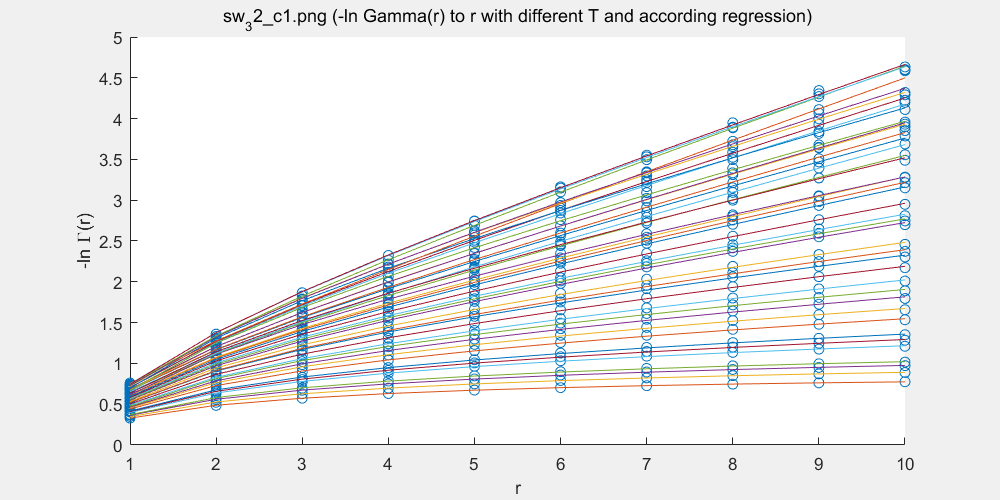
\includegraphics[width=0.45\paperwidth]{pics/sw_32_c1.png}
		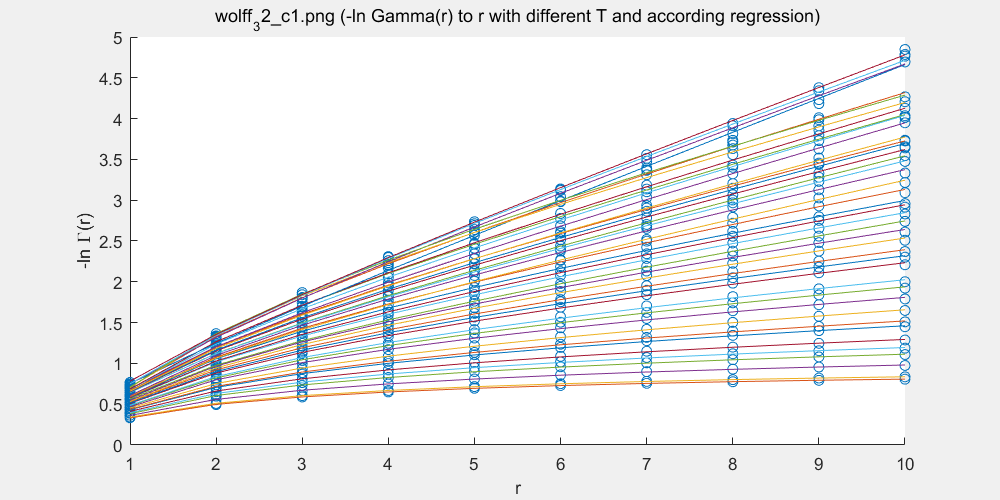
\includegraphics[width=0.45\paperwidth]{pics/wolff_32_c1.png} }
\end{figure}

\begin{figure}[H]
	\centering
	\noindent\makebox[\textwidth][c] {
		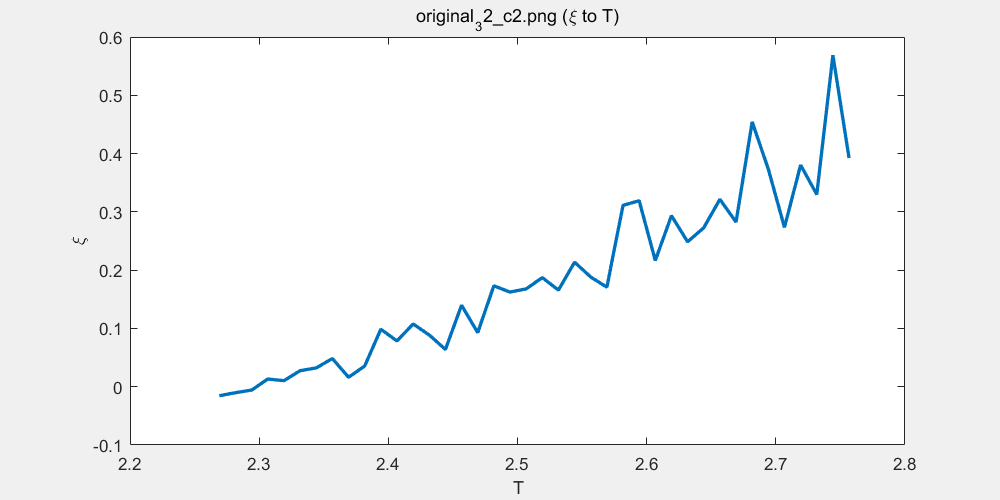
\includegraphics[width=0.45\paperwidth]{pics/original_32_c2.png}
		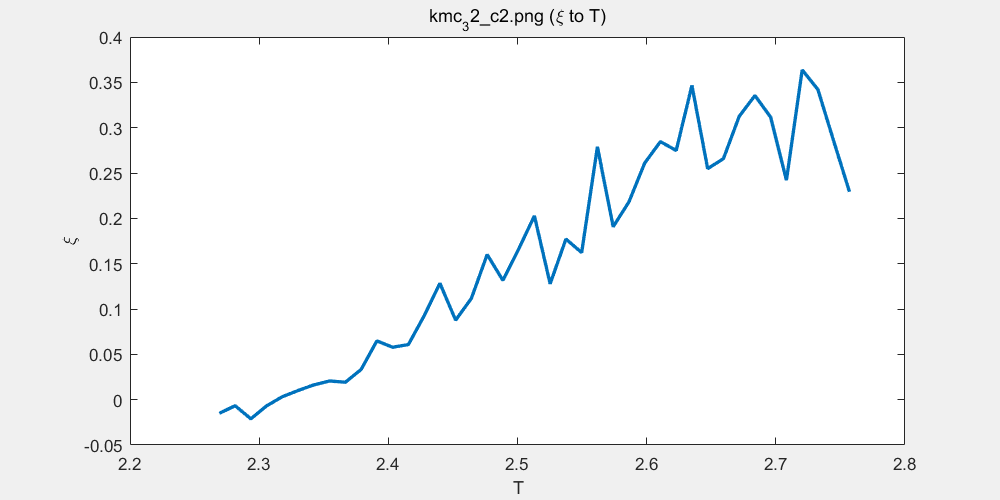
\includegraphics[width=0.45\paperwidth]{pics/kmc_32_c2.png} }
	
	\noindent\makebox[\textwidth][c] {
		\includegraphics[width=0.45\paperwidth]{pics/sw_32_c2.png}
		\includegraphics[width=0.45\paperwidth]{pics/wolff_32_c2.png} }
\end{figure}

\begin{figure}[H]
	\centering
	\noindent\makebox[\textwidth][c] {
		\includegraphics[width=0.45\paperwidth]{pics/original_32_d11.png}
		\includegraphics[width=0.45\paperwidth]{pics/kmc_32_d11.png} }
\end{figure}

\begin{figure}[H]
	\centering
	\noindent\makebox[\textwidth][c] {
		\includegraphics[width=0.45\paperwidth]{pics/original_32_d12.png}
		\includegraphics[width=0.45\paperwidth]{pics/kmc_32_d12.png} }
\end{figure}

\begin{figure}[H]
	\centering
	\noindent\makebox[\textwidth][c] {
		\includegraphics[width=0.45\paperwidth]{pics/original_32_d21.png}
		\includegraphics[width=0.45\paperwidth]{pics/kmc_32_d21.png} }
	
	\noindent\makebox[\textwidth][c] {
		\includegraphics[width=0.45\paperwidth]{pics/sw_32_d21.png}
		\includegraphics[width=0.45\paperwidth]{pics/wolff_32_d21.png} }
\end{figure}

\begin{figure}[H]
	\centering
	\noindent\makebox[\textwidth][c] {
		\includegraphics[width=0.45\paperwidth]{pics/original_32_d22.png}
		\includegraphics[width=0.45\paperwidth]{pics/kmc_32_d22.png} }
	
	\noindent\makebox[\textwidth][c] {
		\includegraphics[width=0.45\paperwidth]{pics/sw_32_d22.png}
		\includegraphics[width=0.45\paperwidth]{pics/wolff_32_d22.png} }
\end{figure}

\begin{figure}[H]
	\centering
	\noindent\makebox[\textwidth][c] {
		\includegraphics[width=0.45\paperwidth]{pics/original_32_d31.png}
		\includegraphics[width=0.45\paperwidth]{pics/kmc_32_d31.png} }
	
	\noindent\makebox[\textwidth][c] {
		\includegraphics[width=0.45\paperwidth]{pics/sw_32_d31.png}
		\includegraphics[width=0.45\paperwidth]{pics/wolff_32_d31.png} }
\end{figure}

\begin{figure}[H]
	\centering
	\noindent\makebox[\textwidth][c] {
		\includegraphics[width=0.45\paperwidth]{pics/original_32_d32.png}
		\includegraphics[width=0.45\paperwidth]{pics/kmc_32_d32.png} }
	
	\noindent\makebox[\textwidth][c] {
		\includegraphics[width=0.45\paperwidth]{pics/sw_32_d32.png}
		\includegraphics[width=0.45\paperwidth]{pics/wolff_32_d32.png} }
\end{figure}


%
%\begin{figure}[htbp]
%	\centering
%	\subfigure[pic1.]{
%		\begin{minipage}[t]{0.25\linewidth}
%			\centering
%			\includegraphics[width=1in]{pics/original_16_a.png}
%			%\caption{fig1}
%		\end{minipage}%
%	}%
%	\subfigure[pic2.]{
%		\begin{minipage}[t]{0.25\linewidth}
%			\centering
%			\includegraphics[width=1in]{pics/original_16_a.png}
%			%\caption{fig2}
%		\end{minipage}%
%	}%
%	\subfigure[pic3.]{
%		\begin{minipage}[t]{0.25\linewidth}
%			\centering
%			\includegraphics[width=1in]{pics/original_16_a.png}
%			%\caption{fig2}
%		\end{minipage}
%	}%
%	\subfigure[pic4.]{
%		\begin{minipage}[t]{0.25\linewidth}
%			\centering
%			\includegraphics[width=1in]{pics/original_16_a.png}
%			%\caption{fig2}
%		\end{minipage}
%	}%
%	\centering
%	\caption{ pics}
%\end{figure}


\end{document}





